%%%%%%%%%%%%%%%%%%%%%%%%%%%%%%%%%%%%%%%%%%%%%%%%%%%%%%%%%%%%%%%%%%%%%%%%%%%%%%%
%%%%%%%%%%%%%%%%%%%%%%%%%%%%%%%%%%%%%%%%%%%%%%%%%%%%%%%%%%%%%%%%%%%%%%%%%%%%%%%
%%%%%%%%%%%%%%%%%%%%%%%%%%%%%%%%%%%%%%%%%%%%%%%%%%%%%%%%%%%%%%%%%%%%%%%%%%%%%%%
%% Marco Sgobino
%% Tesi di laurea triennale

\documentclass[a4paper, 12pt]{report} % Font encoding and italian language support
\usepackage[a-1b]{pdfx}
\usepackage[T1]{fontenc} 
\usepackage[utf8]{inputenc}
\usepackage[italian]{babel}

\usepackage{graphicx} % Manage pictures
\usepackage{hyperref} % Reference Links
\usepackage{times} % Times serif font



\usepackage{color} % Allows defining colors for code snippets
\usepackage{setspace} % Sets leading
\usepackage[a4paper, inner=0.5cm, outer=0.5cm, lmargin=2cm, rmargin=2cm, tmargin=2.5cm, bmargin=2cm]{geometry} % Sets margins and borders


% This will change "\chapter" style into 'N   CHAPTER NAME'
\usepackage{titlesec}

%\usepackage{etoolbox}
%\makeatletter
%\patchcmd{\thebibliography}{%
	%\chapter*{\bibname}\@mkboth{\MakeUppercase\bibname}{\MakeUppercase\bibname}}{%
	%\chapter*{\bibname}}{}{}
%\makeatother




% Code snippets customization
\usepackage{listings}
\definecolor{dkgreen}{rgb}{0.1,0.5,0.1}
\definecolor{greengray}{rgb}{0.32,0.57,0.32}
\definecolor{orange}{rgb}{0.96,0.42,0}
\definecolor{lightblue}{rgb}{0,0.28,0.95}
\definecolor{background}{rgb}{0.995,0.995,0.995}
\lstset {
        frame=tb,
        language=[5.2]Lua,
        aboveskip=3mm,
        belowskip=3mm,
        showstringspaces=false,
        columns=flexible,
        basicstyle={\small\ttfamily},
        numbers=none,
        backgroundcolor=\color{background},
        numberstyle=\tiny\color{drkgeen},
        keywordstyle=\color{lightblue},
        commentstyle=\color{greengray},
        stringstyle=\color{orange},
        breaklines=true,
        breakatwhitespace=true,
        tabsize=3
}

\setlength{\parindent}{28.35pt}


%%%%%%%%%%%%%%%%%%%%%%%%%%%%%%%%%%%%%%%%%%%%%%%%%%%%%%%%%%%%%%%%%%%%%%%%%%%%%%%
%%%%%%%%%%%%%%%%%%%%%%%%%%%%%%%%%%%%%%%%%%%%%%%%%%%%%%%%%%%%%%%%%%%%%%%%%%%%%%%
%%%%%%%%%%%%%%%%%%%%%%%%%%%%%%%%%%%%%%%%%%%%%%%%%%%%%%%%%%%%%%%%%%%%%%%%%%%%%%%

\begin{document}

\begin{titlepage}
        \begin{center}
                \begin{center}
                        
\includegraphics[width=0.15\textwidth, keepaspectratio]{./logo_uniud.jpg}
                \end{center}
                \vspace*{1cm}
                \Large
                \textbf{UNIVERSITÀ DEGLI STUDI DI UDINE}
                \vspace*{1cm}

                \hrule
                \vspace*{0.6cm}

                \large
                Dipartimento Politecnico di Ingegneria ed Architettura

                Corso di Laurea triennale in Ingegneria Elettronica 

                (Cl. L-8)

                \vspace*{2.5cm}

                \large Tesi sperimentale
                \vspace*{0.8cm}

                \Large
                \textbf{SCRIPT LUA PER IL CONTROLLO REMOTO DI DRONI}

                \vfill
                
                \begin{table*}[h]
                        \begin{center}
                                \begin{tabular*}{\textwidth}{@{\extracolsep{\fill}}ll}
                                        \large Relatore: & \large Laureando:  \\
                                                  &             \\
                                        \large Pier Luca Montessoro & \large Marco Sgobino
                                \end{tabular*}
                        \end{center}
                \end{table*}

                \vspace*{1.2cm}
                \hrule
                \vspace*{0.6cm}
                \large
                Anno Accademico 2020-2021

        \end{center}
\end{titlepage}


%\title{Script Lua per controllo remoto droni}
%\author{Marco Sgobino}
%\maketitle % Prints title
\tableofcontents % Prints table of contents
\fontsize{12pt}{14pt}\selectfont % Sets font size
\setstretch{1.5} % Sets leading to 1.5

\titleformat{\chapter}[display]
{\Huge\bfseries}{}{0pt}{\thechapter\ \ \ \ }
%% Frontespizio
%% Indice
\newpage
\clearpage
\chapter{PREMESSA}
Il seguente elaborato di tesi sperimentale si pone l'obiettivo di realizzare degli script in Lua per \emph{OpenTX}, un firmware open source per radiocomandi, con particolare attenzione per i modelli di radiocomando \emph{RadioMaster TX16S} e \emph{Taranis QX7S}. È stato dunque rilevante lo studio della documentazione ufficiale relativa al firmware e al supporto Lua offerto da \emph{OpenTX}. In definitiva, è stato possibile produrre degli script in Lua in grado di estendere le funzionalità in principio messe a disposizione dal firmware dei radiocomandi oggetto di sperimentazione, con uno sviluppo e una sperimentazione interamente effettuati sull'apposito software di simulazione del radiocomando, anch'esso parte integrante di OpenTX.

\clearpage


\chapter{INTRODUZIONE}

OpenTX \cite{opentx-website} è un firmware per radiocomandi, scritto in C++, con supporto per oltre 20 modelli di trasmittenti radio \cite{opentx-radios}.

Il software è rilasciato con licenza \emph{GNU General Public License version 2} ed è dunque integralmente open source \cite{opentx-github}. Lo sviluppo è attualmente in corso ed è gestito da una comunità di sviluppatori e piloti di aeromodelli e droni. Oltre a poter essere scaricato, compilato ed installato nel proprio radiocomando, il firmware è disponibile preinstallato su radiocomandi di vari produttori, fra cui \emph{FrSky} e \emph{RadioMaster}, aziende che hanno realizzato i due modelli adottati nella sperimentazione, il \emph{Taranis FrSky QX7S} ed il \emph{RadioMaster TX16S}.

Il modello di sviluppo open source del software presenta una moltitudine di vantaggi rispetto al modello del software proprietario. Alla base dei progetti, dei prodotti e delle iniziative OSS (Open Source Software) e OSH (Open Source Hardware) vi è lo scambio di informazioni, la cooperazione, la trasparenza, lo sviluppo rapido, la meritocrazia, e miglioramenti orientati alla comunità~\cite{oss-osh-uavs} (Burdziakowski, P., Razmjooy, N., Estrela, V., \& Hemanath, J., 2020). Il software OSS è un software assieme al quale è rilasciato il codice sorgente che chiunque può sottoporre a scrutinio, modificare, e migliorare (Burdziakowski, P., Razmjooy, N., Estrela, V., \& Hemanath, J., 2020).

Poiché i programmatori possono aggiungere funzionalità al codice sorgente di un software open source o modificare parti che non funzionano sempre correttamente, il programma può essere migliorato da chiunque ne sia in grado. Alcuni progetti nell'ambito dei \emph{MAV} (Micro Aerial Vehicles) e della \emph{fotogrammetria} che fanno uso del modello di sviluppo open source sono \emph{Mission Planner} \cite{mission-planner-website}, \emph{Ardupilot} \cite{ardupilot-website}, \emph{OpenDroneMap} \cite{opendronemap}, \emph{Web ODM} \cite{webodm-website} e il firmware \emph{OpenTX} (Burdziakowski, P., Razmjooy, N., Estrela, V., \& Hemanath, J., 2020).

Vi è infatti una serie di ragioni per preferire un modello di sviluppo OSS al posto di un modello di sviluppo proprietario \cite{oss-osh-uavs}, fra le quali vi sono:
\begin{itemize}
        \item il \emph{controllo,} poiché il codice può essere ispezionato e testato con la consapevolezza dovuta alla comprensione del suo funzionamento interno;
        \item l'\emph{addestramento,} dal momento che studenti e programmatori possono liberamente esaminare il codice e condividerlo con altri sviluppatori durante le fasi dello sviluppo, apprendendone da esso il funzionamento ed eventuali errori commessi con una profondità altrimenti impossibile;
        \item la \emph{sicurezza,} poiché il codice liberamente ispezionabile può essere analizzato da esperti di sicurezza e sviluppatori, i quali sono in grado di individuare errori che gli autori originali non hanno identificato. Lo sviluppo più veloce ha come ulteriore e benefica conseguenza la correzione più rapida degli errori rispetto al modello a sorgente proprietario;
        \item la \emph{stabilità,} dal momento in cui il modello OSS tende a sopravvivere nel tempo e ad incorporare standard aperti.
\end{itemize}

L'integrazione degli UAV (Unmanned Aerial Vehicles) nel \emph{remote sensing} in ambito civile sta avendo un impatto sempre più significativo nel settore della fotogrammetria, fotografia, cinematografia, marketing, operazioni di soccorso, ma anche per generiche spedizioni e consegna di materiali in ambito medico e farmaceutico~\cite{rise-uavs} (Cummings, Anthony R.; McKee, Arlo; Kulkarni, Keyur; Markandey, Nakul, 2017). 

L'azienda di ricerche di mercato DOXA Marketing Advice ha compiuto uno studio in Italia relativo all'industria dei droni; nel 2016, questo mercato ha raggiunto livelli record come avvenuto nel 2013, anno nel quale l'ENAC ha introdotto le linee guida per i velivoli a pilotaggio remoto. Nel medesimo studio, viene messo alla luce che le industrie intervistate ritengono che le aree di maggior potenziale per i velivoli a pilotaggio remoto sono l'agricoltura, la fotogrammetria e i rilievi topografici~\cite{italy-uavs} (Andrea Cardamone, 2017).

Dunque, in prospettiva alla crescita del mercato dei velivoli a pilotaggio remoto diviene di estrema importanza l'utilizzo e il contributo a progetti Open Source Software ed Open Source Hardware, al fine di accrescere l'offerta a disposizione sia per il consumatore che per il cliente professionista, nonché di produrre un ambiente di sviluppo collaborativo ove sia possibile includere o progettare degli standard aperti in un ecosistema software gestito da delle comunità di sviluppatori e dalle aziende interessate.


\clearpage

\chapter{MATERIALI E METODI}
\section{Utilizzo e scopo di OpenTX}

Il firmware OpenTX per radiocomandi è composto da due distinte applicazioni\cite{opentx-firmware},
\begin{itemize}
        \item il \emph{System Firmware}, il quale si occupa della gestione e del mantenimento delle impostazioni dell'utente, della lettura degli input dei comandi e delle elaborazioni necessarie al funzionamento del radiocomando;
        \item il \emph{Transmitter Firmware}, responsabile della generazione del segnale radio alla frequenza opportuna e codificato secondo il protocollo supportato dalla radio.
\end{itemize}

La memorizzazione delle informazioni nel radiocomando avviene tramite una memoria di tipo non volatile (ad esempio una memoria a stato solido \emph{SD}), la quale è in grado di immagazzinare i dati di impostazioni, di calibrazione, le informazioni di tutti i modelli, gli script Lua, i suoni, le immagini. Il System Firmware può quindi leggere i dati in memoria e utilizzarli per pilotare il Transmitter Firmware, il quale genererà l'opportuno segnale radio tramite la circuiteria.

Il firmware \emph{OpenTX} dunque si occupa sia di gestire l'input proveniente dagli slider (cursori), stick (leve), switch (interruttori) e knob (manopole) che compongono il telecomando producendo degli output nei 32 canali di trasmissione radio, sia di generare un'interfaccia grafica su uno schermo LCD, con le necessarie schermate di telemetria ed opzioni. Esso consente la configurazione completa della radio, dei modelli salvati in memoria su un supporto SD, o la visualizzazione di telemetria e dati ulteriori, come la batteria residua del radiocomando, la posizione mediante GPS, o l'indicatore \emph{RSSI} della potenza del segnale in ricezione. In aggiunta a ciò, è possibile riprodurre file audio dall'altoparlante della ricetrasmittente per creare annunci personalizzati ed aiutare il pilota con feedback vocali durante le sessioni di volo.


\begin{figure}[ht]
        \centering
        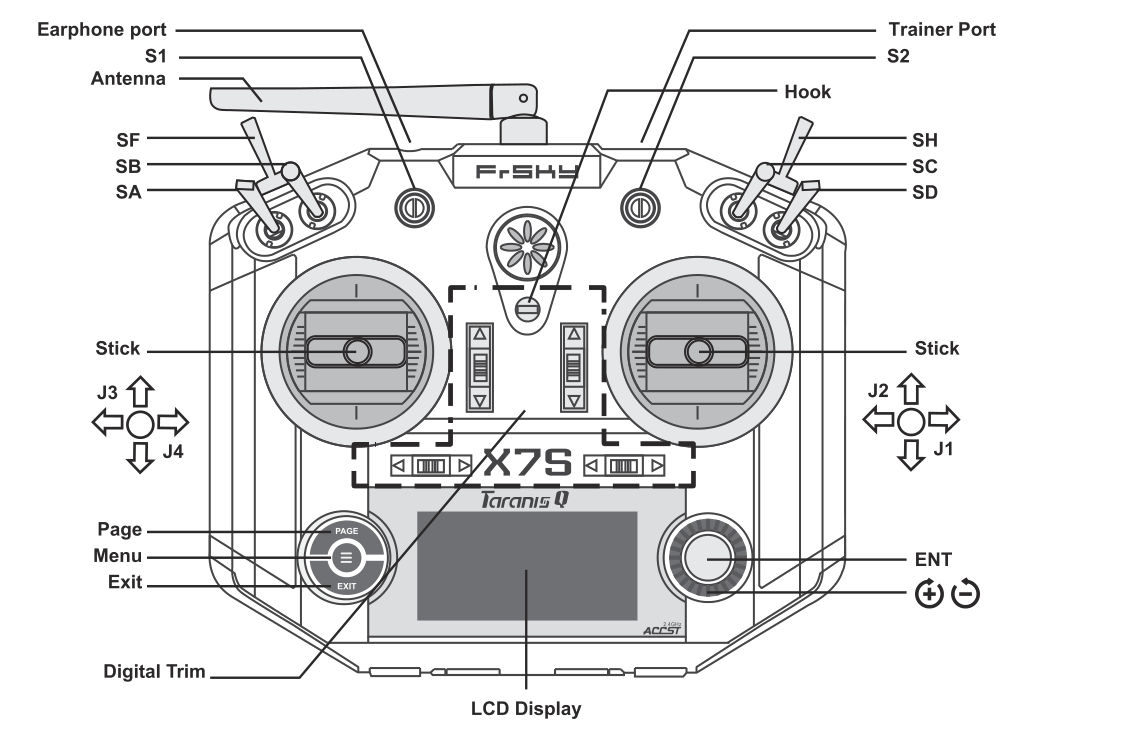
\includegraphics[ width=0.80\linewidth, height=\textheight, keepaspectratio]{./Pictures/qx7s-sticks.png}
        \caption{Leve e cursori del \emph{Taranis QX7S}.}
        \label{fig:qx7s-sticks}
\end{figure}

OpenTX rende inoltre disponibile un software ad interfaccia grafica, \emph{OpenTX Companion} \cite{opentx-website}, disponibile per Windows, macOS e Linux. Tale software velocizza e facilita la configurazione del radiocomando con l'ausilio di un computer e consente di svolgere varie operazioni, fra cui:
\begin{itemize}
        \item scaricare ed installare il firmware OpenTX per il proprio radiocomando;
        \item modificare le configurazioni del radiocomando e dei modelli;
        \item eseguire backup delle configurazioni e ripristinarle all'occorrenza;
        \item modificare la schermata d'avvio del radiocomando;
        \item simulare i radiocomandi ed i modelli tramite il software \emph{OpenTX Simulator}.
\end{itemize}

\subsection{Gestione degli input ed elaborazione degli output mediante i mixer}\label{subsec:inputs-mixers-outputs}

OpenTX gestisce gli input e l'output e la loro elaborazione tramite \emph{cicli di calcolo} eseguiti varie volte al secondo; con ogni ciclo vengono lette le posizioni dei controlli, elaborati i \emph{mixer} e trasmessi gli output nei corretti canali di trasmissione radio. Tutto ciò avviene con sufficiente rapidità da garantire una risposta più rapida possibile alle variazioni degli input e da simulare una continuità nel tempo di tale risposta.

\subsubsection{Le sorgenti}
Le \emph{sorgenti} sono l'insieme delle leve, manopole e cursori che compongono i controlli del radiocomando. L'input viene letto assegnando alla posizione di ciascuno di essi un valore numerico:
\begin{itemize}
        \item un valore continuo da $-100$ a $+100$ per gli stick, gli slider ed i knob. Gli stick sono indicati con \emph{Ele} (Elevator stick), \emph{Ail} (Aileron stick), \emph{Thr} (Throttle stick) e \emph{Rud} (Rudder stick). Quando uno stick è collocato nella sua posizione centrale, il suo valore di input è pari a $0$. I knob invece sono indicati con \emph{S1} ed \emph{S2} (in alcuni radiocomandi con \emph{F1} ed \emph{F2}) e si tratta di manopole la cui funzione può essere liberamente impostata dall'utente. Gli slider di sinistra e destra (LS, RS) sono invece i potenziometri per gli stick, rispettivamente, di sinistra e di destra;
        \item $-100$, $0$ oppure $100$ per gli switch. Sono indicati con \emph{SA, SB, SC} e così via. Sono azionabili su tre posizioni: interruttore al centro (valore $0$), interruttore giù (valore $100$) ed interruttore su (valore $-100$);

        \item $100$ oppure $0$ per gli slider con solo due posizioni (presenti soltanto in alcuni modelli).
\end{itemize}

\subsubsection{I Mixer}
L'input proveniente dalle sorgenti viene elaborato ed inviato ai canali di output attraverso i \emph{mixer}. Ciascun mixer rappresenta l'\emph{interazione fra uno o più input ed uno o più output}. 

Un mixer assegna un input (sorgente) ad un output (canale), elaborandolo mediante varie modalità. OpenTX rende possibile applicare tre diversi tipi di configurazione:
\begin{enumerate}
        \item \emph{da una sorgente ad un canale}: una singola sorgente viene assegnata ad un singolo canale di uscita;
        \item \emph{da una sorgente a canali multipli}: una singola sorgente viene assegnata a più canali di uscita contemporaneamente. Questa configurazione è comune se si intende ad esempio pilotare più alettoni simultaneamente con un unica leva;
        \item \emph{da più sorgenti ad un singolo canale}: gli effetti di più sorgenti vengono sommati in un unico canale di uscita, e ciascuna sorgente fornisce un contributo indipendente al canale di uscita.
\end{enumerate}

\subsubsection{Tipologie di mixer}

I mixer sono in grado di attribuire un \emph{peso} ai valori d'ingresso applicando al valore del segnale un coefficiente espresso con una percentuale, e di assegnare al segnale risultante almeno un canale di output. È possibile creare configurazioni combinando l'azione di più mixer per l'elaborazione dei vari input.

%\begin{minipage}{\textwidth}
Un esempio è quello di impostare gli input dei quattro stick verso $4$ canali di output, facendo in modo che il movimento completo dello stick produca un movimento completo del servo nel modello. Una possibile configurazione per tale scenario fa uso di $4$ mixer, ed è la seguente:

\begin{lstlisting}
        Configurazione dei canali di output
        Canale          Input           Mixer
        CH1             I1:Rud          Weight (+100%)
        CH2             I2:Ele          Weight (+100%)
        CH3             I3:Thr          Weight (+100%)
        CH4             I4:Ail          Weight (+100%)
\end{lstlisting}
%\end{minipage}

Per l'input \texttt{Rud} è stato assegnato l'output nel canale \texttt{CH1} con peso \texttt{+100\%}, per l'input \texttt{Ele} è stato assegnato l'output nel canale \texttt{CH2} anch'esso con peso \texttt{+100\%}, e così via per gli altri due input \texttt{Thr} ed \texttt{Ail}.

Opzioni alternative possono essere quelle di ridurre l'effetto dei singoli stick, dando ad essi un peso minore (ad esempio la metà, $50\%$), oppure invertire il segno del peso di modo da produrre un movimento del servo nella direzione opposta.

È inoltre possibile impostare un \emph{offset} per il valore in uscita, mediante la formula
$$\mbox{output } = \mbox{ sorgente} \cdot \mbox{peso } + \mbox{ offset }.$$

In aggiunta ai \emph{pesi} e agli \emph{offset}, OpenTX consente di valutare le sorgenti attraverso varie funzioni più complesse:
\begin{itemize}
        \item \emph{Diff}: riduce l'effetto dello stick in una direzione del movimento, applicando un peso, specificato in percentuale;
        \item \emph{Expo}: applica una curva esponenziale al segnale di input;
        \item \emph{Function}: applica una funzione matematica, o una disuguaglianza al segnale. Le funzioni sono in grado, ad esempio, di fornire in uscita il valore assoluto del segnale d'ingresso, oppure di prelevare l'input soltanto nel caso esso sia positivo $(x>0)$;
        \item \emph{Curve}: applica una curva impostata dall'utente. Esse sono configurabili assegnando manualmente il valore della curva in alcuni punti, il cui numero varia da $2$ a $17$.
\end{itemize}




\section{Supporto OpenTX per gli script Lua}

Con la versione 2.0~\cite{opentx-lua-instructions} OpenTX ha introdotto il supporto al \emph{Lua}, un linguaggio di scripting general-purpose \cite{lua-website}. Gli script Lua sono immagazzinati nella memoria SD, tipicamente al percorso \texttt{/SCRIPTS/} con un nome massimo di 6 caratteri, esclusa l'estensione. Gli script Lua sono eseguiti dal firmware automaticamente o a discrezione dell'utente a seconda della tipologia dello script.

Gli script in Lua sono suddivisi in due categorie maggiori: gli \emph{one-time script} o \emph{script monouso}, e gli \emph{script persistenti}.

\subsubsection{Script persistenti}
Si tratta degli script caricati dal firmware all'avvio, che rimangono in esecuzione fino a quando il radiocomando è in funzione oppure fino a quando viene selezionato un modello differente. Il firmware rende limitato l'utilizzo della memoria RAM da parte degli script Lua, pertanto è possibile eseguire contemporaneamente \emph{fino ad un massimo di 7 script persistenti}. Il firmware inoltre si occupa della gestione della memoria e delle disponibilità di calcolo, interrompendo l'esecuzione di qualsiasi script che impieghi una quantità eccessiva di risorse.

Vi sono più tipi di script persistenti:
\begin{itemize}
        \item gli \emph{script di modello} o \emph{model script}: sono eseguiti dal momento in cui viene selezionato un modello fino a quando esso viene deselezionato. Gli script di modello vengono anche detti \emph{mixes script} poiché svolgono una funzione analoga, sebbene più avanzata, dei mixer in precedenza descritti nella sezione~\ref{subsec:inputs-mixers-outputs}. Essi permettono dunque di elaborare un input o una serie di input restituendo un singolo valore o una table in output;

        \item gli \emph{script di funzione} o \emph{function script}: sono analoghi ai precedenti script di modello, con la differenza che essi vengono eseguiti quando una condizione su un interruttore o una leva si verifica (ad esempio, un interruttore viene azionato). Lo script viene ugualmente precaricato all'avvio del modello, e resta in attesa del verificarsi della condizione per cui esso è invocabile. Essi dunque svolgono un ruolo analogo a quello dei mixer, ma successivamente al verificarsi di una condizione. Possono anche gestire annunci vocali ed allarmi personalizzati, ma non sono in grado di stampare stringhe o valori numerici su schermo;

        \item gli \emph{script di telemetria} o \emph{telemetry script}: lo scopo di questi script è quello di presentare al pilota dati di volo e informazioni sullo stato del modello sulle apposite schermate di telemetria. Sono in grado di interagire e modificare con la schermata del radiocomando. Possono inoltre riprodurre annunci vocali;

        \item i \emph{widget}: sostituiscono gli script di telemetria, di cui sono l'evoluzione, nei modelli di radiocomandi più avanzati (ad esempio il \emph{RadioMaster TX16S}). Essi vengono caricati ed eseguiti quando sono selezionati dalla schermata dei widget. Svolgono le stesse funzioni degli script di telemetria presentando maggiori funzionalità: oltre alla possibilità di interagire con la schermata e di stampare su schermo stringhe testo e figure, sono in grado di assumere una dimensione e collocazione sullo schermo variabile, con la facoltà di collocarne più di uno per schermata. Essi forniscono inoltre all'utente la capacità di modificarne parametri e variabili mediante un menù delle opzioni direttamente accessibile dall'interfaccia del radiocomando.
\end{itemize}

\subsubsection{One-time script}
        Sono script invocati da una specifica funzione della radio oppure dall'utente tramite un menù contestuale. L'esecuzione di uno one-time script disabilita temporaneamente l'esecuzione di tutti gli altri script persistenti liberando la memoria RAM per lo script monouso. Gli script persistenti vengono poi ripristinati al termine dell'esecuzione dello one-time script. Gli one-time script possono essere adoperati per creare dei programmi di installazione o configurazione di modelli con interfaccia grafica direttamente dalla radio.

\subsection{Struttura di uno script di modello}\label{subsec:struttura-script-modello}
I \emph{model script} sono eseguiti dal firmware successivamente al caricamento del modello nelle impostazioni del radiocomando. L'esecuzione non cessa mai fino alla selezione di un nuovo modello. Essi sono eseguiti con priorità \emph{inferiore} rispetto ai mixer integrati visti nella sezione~\ref{subsec:inputs-mixers-outputs}, e presentano un periodo di esecuzione dell'ordine dei $30ms$. La loro esecuzione è secondaria rispetto ai mixer, e a seconda delle disponibilità di risorse di calcolo e di memoria può non essere garantita.

La struttura di uno script di modello è la seguente:
\begin{itemize}
        \item funzione \texttt{init()} (opzionale): eseguita una singola volta all'avvio dello script. Essa può essere adoperata per eseguire operazioni iniziali all'avvio dello script;
        \item funzione \texttt{run()}: eseguita periodicamente, essa può opzionalmente ricevere degli argomenti e restituire dei valori;
        \item tabella \texttt{input} (opzionale): table contenente uno o più elementi corrispondenti agli input dello script;
        \item tabella \texttt{output} (opzionale): table contenente uno o più elementi corrispondenti agli output dello script;
        \item statement \texttt{return}: collocato alla fine del codice, restituisce una tabella a cui associamo agli elementi \texttt{run}, \texttt{init}, \texttt{input} ed \texttt{output} le stringhe dei nomi delle corrispondenti funzioni o tabelle. Con esso si compie l'associazione fra le funzioni o variabili riconosciute dal firmware (\texttt{run()}, \texttt{init()}, \texttt{input}, \texttt{output}) con i nomi delle corrispondenti funzioni nello script, arbitrariamente scelti dall'utente.
\end{itemize}

La funzione \texttt{run()} non richiede parametri di input ed il return all'interno di essa è opzionale. La struttura di un model script con la sola funzione \texttt{run()}, a cui è stato assegnato il nome di \texttt{esegui\_calcoli()}, sarà dunque la seguente:

\begin{lstlisting}
local function esegui_calcoli()
        -- Esegui calcoli periodicamente
end

return { run=esegui_calcoli }   -- esegui_calcoli e' ora
        -- associata alla funzione run() dello script
\end{lstlisting}

Le tabelle opzionali dei valori di input e di output contengono la stringa con il nome dei corrispondenti valori di ingresso ed uscita e vengono mostrate direttamente dall'interfaccia grafica del radiocomando, con a fianco il corrispondente valore. Per essi, OpenTX supporta la visualizzazione su schermo di nomi con lunghezza fino ad 8 caratteri. Gli ingressi di un model script possono essere più di uno, fino ad un totale di 6, e sono di due tipi:
\begin{itemize}
        \item \texttt{VALUE}: valore numerico. Esso fornisce un valore costante in ingresso, definibile dall'utente mediante l'interfaccia grafica. La sua sintassi è una tabella in Lua del tipo 
\begin{lstlisting}
{ "Nome", VALUE, <minimo>, <massimo>, <predefinito> }
\end{lstlisting}
        \item \texttt{SOURCE}: sorgente di input da cui prelevare il segnale. Le sorgenti possono essere canali, interruttori, valori di telemetria, stick, e così via. La sintassi per le sorgenti è la seguente:
\begin{lstlisting}
{ "Nome", SOURCE }
\end{lstlisting}
\end{itemize}

Un esempio più completo di struttura di un model script a 2 ingressi e 3 uscite è il sottostante:

\begin{lstlisting}
local ingressi = {
        { "Sorgente", SOURCE}, -- Sorgente di input
        { "Numero", VALUE, 0, 100, 50} -- Valore numerico
                                -- compreso fra 0 e 100, e con 
                                -- valore predefinito 50
}
-- contiene le stringhe dei nomi dei valori d'uscita
local uscite = { 
        "Valore1:",
        "Valore2:",
        "Valore3:"
}
local function inizializza()
        -- Esegui operazioni all'avvio
        -- dello script
end
local function esegui_calcoli(sorgente_ingresso, numero)
        -- Gli ingressi della funzione esegui_calcoli
        -- sono rispettivamente i valori 
        -- della table "ingressi"

        -- Esegui calcoli periodicamente
        
        return valore_uno, valore_due, valore_tre
        -- Questi valori sono restituiti
        -- in questo ordine
        -- nella table "uscite"
end
return { run=esegui_calcoli, init=inizializza, input=ingressi, output=uscite }
\end{lstlisting}

La funzione \texttt{esegui\_calcoli(sorgente\_ingresso, numero)} ha due variabili come suoi argomenti. Esse sono automaticamente prelevate, in ordine di dichiarazione, dalla table \texttt{ingressi}, perciò a \texttt{sorgente\_ingresso} verrà associato il valore dell'input ``Sorgente'', il primo presente nella table \texttt{ingressi}, mentre a \texttt{numero} verrà associato il valore dell'input ``Numero'', dichiarato successivamente. Similmente, nell'istruzione di \texttt{return} sono restituiti tre valori: il primo, \texttt{valore\_uno}, sarà associato all'uscita ``Valore1'', il secondo, \texttt{valore\_due}, all'uscita ``Valore2'', ed infine \texttt{valore\_tre} sarà associato all'uscita ``Valore3''.

Nel frammento di codice sopra si evidenzia come tutte le variabili, comprese le definizioni di funzioni, siano dichiarate come \emph{variabili locali}. Eventuali variabili dichiarate non localmente sarebbero infatti visibili agli altri script in esecuzione nell'ambiente Lua di OpenTX, con possibilità di generare errori o interazioni fra script impreviste dovute all'utilizzo improprio della stessa variabile da parte di più script. I file \texttt{.lua} degli script di modello vanno collocati al percorso \texttt{/SD/SCRIPTS/MIXES}.
I casi d'uso tipici di un model script sono:
\begin{itemize}
        \item sostituzione di mixer complessi e non critici per il funzionamento del modello;
        \item elaborazione complessa di input e sorgenti e riproduzione di annunci vocali in relazione al loro comportamento;
        \item filtraggio di valori di telemetria.
\end{itemize}



\subsection{Struttura di uno script di telemetria}
Gli elementi di uno script di telemetria sono i seguenti:
\begin{itemize}
        \item funzione \texttt{init()} (opzionale): viene eseguita all'avvio dello script di telemetria;
\begin{lstlisting}
local function inizializza()
        -- Esegui operazioni all'avvio
end
\end{lstlisting}
        \item funzione \texttt{run()}: viene eseguita periodicamente, solamente quando la schermata di telemetria è visibile;
\begin{lstlisting}
local function funzione_run()
        -- Esegui operazioni quando
        -- la schermata e' visibile
end
\end{lstlisting}
        \item funzione \texttt{background()} (opzionale): viene eseguita periodicamente, sia quando la schermata di telemetria è visibile che quando è nascosta;
\begin{lstlisting}
local function funzione_background()
        -- Esegui operazioni sia quando
        -- la schermata e' visibile che
        -- quando la schermata e' nascosta
end
\end{lstlisting}

        \item statement \texttt{return}: restituisce la tabella a cui associamo agli elementi \texttt{run}, \texttt{background} e \texttt{init} le stringhe dei nomi delle corrispondenti funzioni o tabelle.
\begin{lstlisting}
return { run=funzione_run, background=funzione_background, init=inizializza }
\end{lstlisting}
\end{itemize}

Dunque, le funzioni \texttt{run()} e \texttt{background()} svolgono un ruolo analogo a quanto osservato per la funzione \texttt{run()} degli script di modello, con la differenza che la loro chiamata dipende dalla schermata che viene visualizzata sul display del radiocomando. In aggiunta, esse hanno la facoltà di modificare l'interfaccia della radio nelle apposite schermate di telemetria e di stampare su schermo stringhe e valori.

Gli script di telemetria vengono caricati appena il modello è selezionato dai menù della radio. Viene inizialmente eseguita, se presente, la funzione \texttt{init()}, e al termine di essa sono periodicamente chiamate le funzioni \texttt{run()} e \texttt{background()} a seconda che sia mostrata la schermata di telemetria o una schermata differente\footnote{\scriptsize Nel caso in cui sia mostrata la schermata di telemetria, vengono eseguite in alternanza sia la funzione \texttt{run()} che la funzione \texttt{background()}.}.

%\begin{minipage}{\textwidth}
A seconda della complessità dello script, potrebbe risultare conveniente consentire all'utente di configurare lo script di telemetria secondo le proprie esigenze. La configurazione degli script di telemetria non avviene mediante interfaccia grafica. La soluzione adottata è quella di dichiarare opportune variabili di configurazione nella parte iniziale dello script, il cui valore è da assegnare direttamente nel codice mediante un editor di testo:

\begin{lstlisting}
-- Eventuali variabili di configurazione
-- il cui valore e' assegnato direttamente nel codice
local VARIABILE_DI_CONFIGURAZIONE = 0
local ALTRA_VARIABILE = 100
\end{lstlisting}
%\end{minipage}

La collocazione degli script di telemetria nella scheda SD è al percorso \texttt{/SCRIPTS/TELEMETRY/}. 
I tipici casi d'uso degli script di telemetria possono essere:
\begin{itemize}
        \item stampa su schermo di stringhe e dati di telemetria;
        \item riproduzione di annunci vocali personalizati;
        \item rappresentazione su schermo mediante figure e numeri di dati di telemetria.
\end{itemize}



\subsection{Struttura di uno script Widget}
I widget sono una variante più complessa degli script di telemetria. La loro struttura è la seguente:
\begin{itemize}
        \item stringa \texttt{name}: il nome del widget (massimo 10 caratteri). Essa è dichiarata come variabile locale o passata direttamente tramite il \texttt{return} alla fine del codice;
        \item funzione \texttt{create()}: viene chiamata una singola volta alla selezione del widget dal menù del radiocomando. Crea il widget, e si occupa di passare alle altre funzioni presenti nello script le \emph{dimensioni} (dette \texttt{zone}) del widget e la table \texttt{options} delle opzioni;
\begin{lstlisting}
local function create (zone, options)
        -- Assegno al widget la zona e le opzioni
        -- ricevute come argomento dal firmware
        local widget = { zone=zone, options=options }
        return widget
end
\end{lstlisting}
        \item funzione \texttt{update()}: viene chiamata ogni volta che un'opzione presente nel menù contestuale del radiocomando viene modificata. Essa aggiorna la table delle opzioni con la nuova tabella passata dal firmware;
\begin{lstlisting}
local function update(widget, options)
        -- Verifico che il widget
        -- sia stato modificato
        -- correttamente
        if (widget ~= nil) then
                widget.options = options
        end
end
\end{lstlisting}
        \item funzione \texttt{refresh()}: eseguita periodicamente, solo quando la schermata di telemetria è visibile;
\begin{lstlisting}
local function refresh(widget)
        -- Esegui operazioni periodicamente
end
\end{lstlisting}
        \item funzione \texttt{background()}: eseguita periodicamente quando il widget non è visibile nella schermata. Si osservi che il comportamento di questa funzione differisce dal comportamento presentato dalla funzione \texttt{background()} degli script di telemetria, in quanto essa viene invocata solo quando il widget non è presente sulla schermata, e non più anche quando esso è visibile;
\begin{lstlisting}
local function background(widget)
        -- Esegui operazioni periodicamente quando non e' visibile
end
\end{lstlisting}
        \item table \texttt{options}: tabella delle opzioni configurabili dal pilota tramite l'interfaccia grafica. Esse presentano una sintassi del tutto simile alla tabella \texttt{input} degli script di modello;
\begin{lstlisting}
local options = {
        { "Color", COLOR, BLUE }, 
        { "Number", VALUE, 10, 1, 100 },
        { "Flag", BOOL, 0 } 
}
\end{lstlisting}
        \item statement \texttt{return}: restituisce la tabella a cui associamo agli elementi \texttt{name}, \texttt{create},  \texttt{update}, \texttt{refresh}, \texttt{background} ed \texttt{options} le stringhe dei nomi delle corrispondenti funzioni o tabelle analogamente a quanto avveniva per gli script di telemetria o gli script di modello.
\begin{lstlisting}
return { name="NomeWidget",
        options=options,
        create=create,
        update=update,
        background=background,
        refresh=refresh }
\end{lstlisting}
\end{itemize}

I possibili tipi di dato utilizzabili nelle opzioni sono \texttt{VALUE}, \texttt{SOURCE}, \texttt{BOOL} e \texttt{COLOR}. In particolare:
\begin{itemize}
        \item \texttt{VALUE}: valore numerico. Esso fornisce un valore costante, definibile dall'utente mediante l'interfaccia grafica. La sua sintassi è una tabella in Lua del tipo:
\begin{lstlisting} 
{ "Nome", VALUE, <predefinito>, <minimo>, <massimo> }
\end{lstlisting}
        \item \texttt{SOURCE}: sorgente di input da cui prelevare il valore. Le sorgenti possono essere canali, interruttori, valori di telemetria, stick, e così via. La sintassi per le sorgenti è la seguente: 
\begin{lstlisting} 
{ "Nome", SOURCE } 
\end{lstlisting}
        \item \texttt{BOOL}: variabile booleana avente possibili valori \texttt{0} (vero) ed \texttt{1} (falso). La sintassi è la table:
\begin{lstlisting}
{ "Nome", BOOL, <vero/falso> }
\end{lstlisting}
        \item \texttt{COLOR}: variabile che contiene un colore, principalmente utilizzata per impostare il colore in cui verranno stampati testo, elementi dell'interfaccia o sfondo del widget. È utilizzata all'interno di una table avente formato:
\begin{lstlisting} 
{ "Nome", COLOR, <rgb> } 
\end{lstlisting} 
        I colori sono espressi in formato \texttt{RGB565}, oppure è possibile assegnare i colori predefiniti dal firmware \texttt{WHITE}, \texttt{GREY}, \texttt{LIGHTGREY}, \texttt{DARKGREY}, \texttt{BLACK}, \texttt{YELLOW}, \texttt{BLUE}, \texttt{RED} e \texttt{DARKRED}.
\end{itemize}

I widget vanno collocati nel percorso \texttt{/WIDGETS/<NomeWidget>/main.lua}, ovverosia come un file di nome \texttt{main.lua} e dentro una cartella avente lo stesso nome di quello assegnato al widget e indicato all'interno dello script.

\subsection{Interazione con il display del radiocomando}
Gli script di telemetria e i widget offrono la possibilità di interagire con il display LCD del radiocomando. L'accesso è limitato, ed è esclusivo delle funzioni \texttt{run()} degli one-time script e telemetry script, e della funzione \texttt{refresh()} dei widget.
Le caratteristiche del display LCD variano profondamente a seconda del modello di radiocomando utilizzato. Gli script in Lua che si interfacciano con l'utente tramite il display devono essere progettati tenendo conto delle caratteristiche dello schermo LCD dei vari modelli. In questo elaborato esporremo le caratteristiche dello schermo dei due modelli adoperati, il \emph{Taranis QX7S} ed il \emph{RadioMaster TX16S}. 

\subsubsection{Display LCD del Taranis QX7S}
Il display LCD del \emph{Taranis} ha una risoluzione di $128\times64$ pixel e supporta $1$ bit di colore. La schermata si presenta come in Figura~\ref{fig:taranis-lcd-screenshot}.

\begin{figure}[ht]
        \centering
        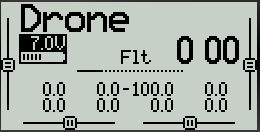
\includegraphics[ width=0.70\linewidth, height=\textheight, keepaspectratio]{./Pictures/taranis-lcd-screenshot.png}
        \caption{Schermata principale del \emph{Taranis QX7S}.}
        \label{fig:taranis-lcd-screenshot}
\end{figure}

La schermata a due colori (chiaro e scuro) rende possibile la lettura di scritte e semplici figure. 

\subsubsection{Display LCD del RadioMaster TX16S}
Il display LCD del \emph{RadioMaster} ha una risoluzione di $480\times272$ pixel e supporta la modalità di colore \texttt{RGB565}. La schermata principale si presenta come in Figura~\ref{fig:radiomaster-lcd-screenshot}. Si può osservare che lo schermo, diversamente dal \emph{Taranis}, supporta una modalità a colori avanzata. La risoluzione è infatti sufficiente per visualizzare figure complesse e scritte di varie dimensioni e colore.
\clearpage

\begin{figure}[hbt]
        \centering
        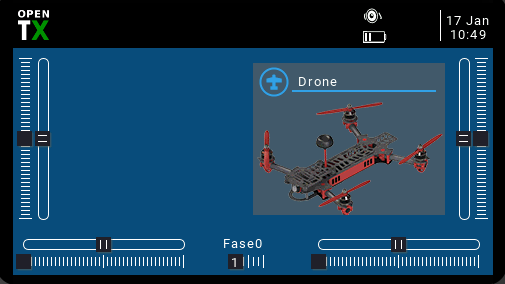
\includegraphics[ width=0.70\linewidth, height=\textheight, keepaspectratio]{./Pictures/radiomaster-lcd-screenshot.png}
        \caption{Schermata principale del \emph{RadioMaster TX16S}.}
        \label{fig:radiomaster-lcd-screenshot}
\end{figure}

\subsubsection{Gestione dello schermo mediante le funzioni \texttt{lcd}}\label{section:funzioni-lcd}
L'ambiente Lua di OpenTX mette a disposizione dei metodi interni all'oggetto \texttt{lcd} in grado di gestire lo schermo LCD del radiocomando, fornendo un'interfaccia tra di esso ed lo script in Lua. Tali metodi possono essere invocati soltanto dai tipi di script per cui è prevista la possibilità di modificare lo schermo, ovvero dagli \emph{one-time script}, dai \emph{telemetry script} e dai \emph{widget} per i radiocomandi che li supportano.

\begin{table}[ht]
        \begin{center}
                \begin{tabular}{|l|r|}
                        \hline
                        \textbf{FLAG} & \textbf{Descrizione}\\
                        \hline
                        \hline
                        \texttt{0} & Testo normale, nessuna cifra decimale\\
                        \hline
                        \texttt{DBLSIZE} & Testo a dimensione doppia\\
                        \hline
                        \texttt{MIDSIZE} & Testo a dimensione intermedia\\
                        \hline
                        \texttt{SMLSIZE} & Testo a dimensione piccola\\
                        \hline
                        \texttt{INVERS} & Colore di testo e sfondo invertito\\
                        \hline
                        \texttt{BLINK} & Testo lampeggiante\\
                        \hline
                        \texttt{XXLSIZE} & Testo a dimensione molto grande\\
                        \hline
                        \texttt{LEFT} & Testo giustificato a sinistra\\
                        \hline
                        \texttt{RIGHT} & Testo giustificato a destra\\
                        \hline
                        \texttt{PREC1} & Singola cifra decimale per i numeri\\
                        \hline
                        \texttt{PREC2} & Doppia cifra decimale per i numeri\\
                        \hline
                        \texttt{GREY\_DEFAULT} & Lo sfondo del testo è grigio\\
                        \hline
                        \texttt{TIMEHOUR} & Mostra le ore\\
                        \hline
                \end{tabular}
        \end{center}
        \caption{Lista dei possibili flag per i metodi dell'oggetto \texttt{lcd}.}
        \label{tab:elenco-flag-lcd}
\end{table}

I metodi che sono stati adoperati per la gestione dell'interfaccia grafica nella realizzazione degli script sono i seguenti:
\begin{itemize}
        \item \texttt{lcd.clear([color])}: metodo utilizzato negli script di telemetria per resettare la schermata prima di effettuare operazioni di stampa su schermo. Il comando accetta come argomento, opzionalmente, un colore con cui effettuare l'azzeramento della schermata, qualora lo schermo supportasse la modalità a colori. Tale metodo non è necessario negli script widget;
        \item \texttt{lcd.drawText(x, y, text, [flags])}: stampa su schermo la stringa di testo \texttt{text}, alla posizione orizzontale \texttt{x} e verticale \texttt{y}. L'elenco dei \texttt{flag} disponibili è indicato in tabella~\ref{tab:elenco-flag-lcd};
        \item \texttt{lcd.drawTimer(x, y, value, [flags])}: stampa su schermo un timer con valore in secondi \texttt{value}, alla posizione orizzontale \texttt{x} e verticale \texttt{y}. L'elenco dei \texttt{flag} disponibili è indicato in tabella~\ref{tab:elenco-flag-lcd};
        \item \texttt{lcd.drawScreenTitle(title, page, pages)}: stampa su schermo il titolo della schermata \texttt{title}, al numero di pagina \texttt{page} e con numero totale di pagine \texttt{pages};
        \item \texttt{lcd.setColor(area, color)}: per gli schermi in grado di supportare i colori, assegna un colore \texttt{color} alla porzione di schermo indicata dalla costante \texttt{area}. In questo elaborato, per il valore di \texttt{area} è stata utilizzata la costante \texttt{CUSTOM\_COLOR};
        \item \texttt{lcd.drawFilledRectangle(x, y, w, h, [flags])}: disegna un rettangolo pieno, alla posizione orizzontale \texttt{x} e verticale \texttt{y} e di ampiezza \texttt{w} ed altezza \texttt{h}. L'elenco dei \texttt{flag} disponibili è indicato in tabella~\ref{tab:elenco-flag-lcd}.
\end{itemize}










\section{OpenTX Companion}

\emph{OpenTX Companion} è un software di supporto per il firmware OpenTX, sviluppato dal medesimo gruppo di sviluppatori che si occupa del firmware. Esso è un programma scritto in C++ e sviluppato per Linux, macOS e Windows che consente la configurazione del radiocomando direttamente da computer, senza incorrere nelle limitazioni imposte dalla dimensione della schermata della radio e dai suoi pulsanti. OpenTX Companion è infatti adoperato per svolgere agevolmente vari compiti, fra i quali il caricamento del firmware sul radiocomando, eseguire il backup delle impostazioni dei modelli, della scheda SD e del firmware, modificare le configurazioni del radiocomando e condurre delle simulazioni del radiocomando \cite{opentx-companion-manual}. Quest'ultimo compito è svolto grazie al simulatore \emph{OpenTX Simulator}, incluso nel software Companion.

\subsection{Specifiche e compilazione del sorgente}
Per questo elaborato è stato adoperato il sistema operativo Fedora Linux 33 \cite{fedora-website}, con la versione 2.3.11 di OpenTX Companion compilata da codice sorgente.
La compilazione del software è avvenuta dapprima installando le necessarie dipendenze, successivamente clonando il repository di \texttt{opentx} ed infine eseguendo lo script di compilazione \texttt{build-companion-release.sh}. Sono stati eseguiti i seguenti comandi (in bash):

\begin{lstlisting}
# Installazione delle dipendenze
sudo dnf -y install sed make cmake git gcc gcc-c++ gcc-arm-linux-gnu avr-gcc-c++ avr-gcc xsd bc python python3-pyqt4-sip PyQt4-qsci-api python3-PyQt4-devel python3-pillow python3-pillow-devel avr-libc qt5-qttools qt5-qttools-devel qt5-qtmultimedia qt5-qtmultimedia-devel qt5-linguist qt5-qtsvg qt5-qtsvg-devel dfu-util gcc-plugin-devel fox fox-devel fox-utils SDL SDL-devel SDL2 SDL2-devel SDL_sound sdljava arm-none-eabi-gcc-cs arm-none-eabi-gcc-cs-c++ arm-none-eabi-newlib rpmdevtools rpm-build

# Clone del repository
git clone --recursive -b 2.3 https://github.com/opentx/opentx.git
cd opentx

# Script per la compilazione
./tools/build-companion-release.sh ../ ./build 23
\end{lstlisting}

Al termine dell'esecuzione dell'ultimo comando, OpenTX sarà correttamente compilato all'interno della cartella \texttt{build}. Sarà possibile eseguire il programma con \texttt{./build/companion23}.

Alternativamente, è fornito un eseguibile per Windows, Ubuntu o macOS nella relativa pagina web di download \cite{opentx-download-page}.

\subsection{Utilizzo e funzionalità}

\begin{figure}[ht]
        \centering
        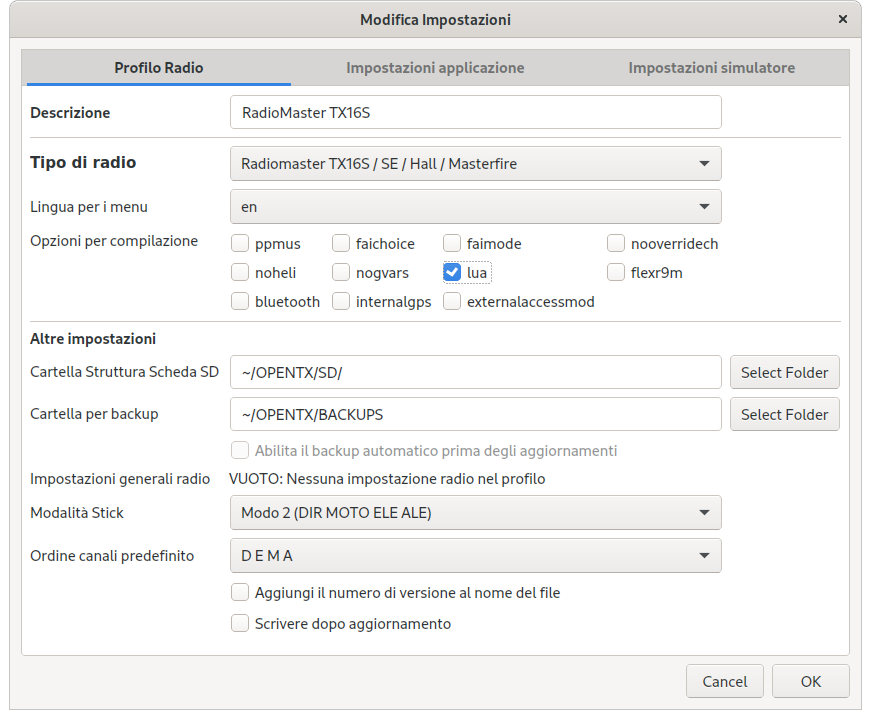
\includegraphics[ width=0.80\linewidth, height=\textheight, keepaspectratio]{./Pictures/opentx-first-config.png}
        \caption{Finestra di prima configurazione di OpenTX Companion.}
        \label{fig:opentx-first-config}
\end{figure}

Al primo avvio di OpenTX Companion è presente una finestra introduttiva, dove viene richiesta una prima configurazione di un profilo di radiocomando. Si seleziona il modello di radiocomando desiderato, nel nostro caso \emph{Taranis QX7S} oppure \emph{RadioMaster TX16S}, e si assegna una breve descrizione al profilo. Successivamente, si include il supporto agli script Lua selezionando la relativa casella e si indica il percorso dove verranno collocati i contenuti della scheda SD, ed opzionalmente, il percorso per i backup. Le restanti impostazioni sono lasciate ai loro valori predefiniti.

\clearpage

La schermata principale di OpenTX Companion si presenta come in Figura~\ref{fig:opentx-main}. Prima di poter simulare un modello, è necessario scaricare il firmware e i contenuti della scheda SD. Per fare ciò, si naviga sull'icona di ``Download'' nella barra degli strumenti per procedere con lo scaricamento. I contenuti della scheda SD andranno poi decompressi con un programma di gestione di file \texttt{.zip} e collocati nella posizione precedentemente indicata.

\begin{figure}[ht]
        \centering
        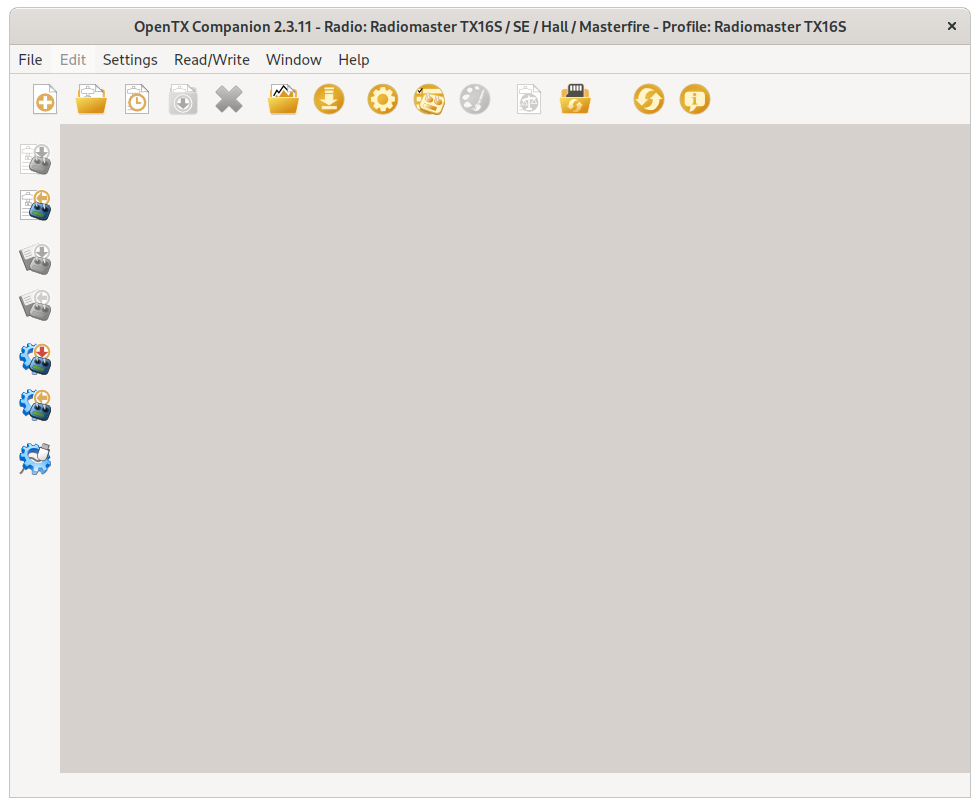
\includegraphics[ width=0.80\linewidth, height=\textheight, keepaspectratio]{./Pictures/opentx-main.png}
        \caption{Finestra principale di OpenTX Companion.}
        \label{fig:opentx-main}
\end{figure}

Prima di simulare il proprio radiocomando è necessario creare un nuovo documento in OpenTX, e collocarvi almeno un modello. Si naviga sull'icona ``New'' nella barra degli strumenti e si aggiunge un nuovo modello con ``Add Model'' all'interno della finestra che è stata aperta. Il Wizard di configurazione del modello guiderà l'utente nella selezione delle sue specifiche. È possibile configurare ulteriormente le opzioni della radio in ``Edit Radio Settings'' prima di lanciare la simulazione. In tale menù è possibile applicare varie configurazioni, calibrazioni e funzionalità specifiche come la possibilità di implementare delle \emph{Global Functions}, azioni da eseguire al verificarsi di un evento (ad esempio, una leva è in una determinata posizione o il pilota aziona un determinato bottone).

\clearpage


\begin{figure}[ht]
        \centering
        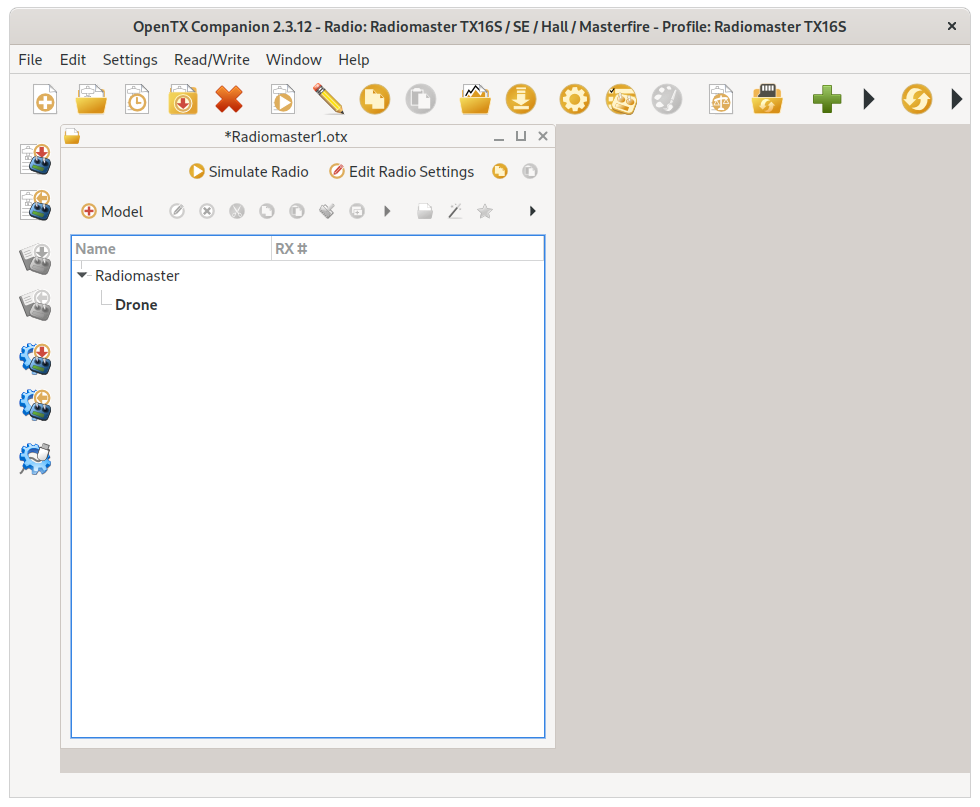
\includegraphics[ width=0.80\linewidth, height=\textheight, keepaspectratio]{./Pictures/opentx-document.png}
        \caption{Creazione di un documento in OpenTX Companion.}
        \label{fig:opentx-document}
\end{figure}

Terminata la configurazione, è possibile eseguire la simulazione con \emph{OpenTX Simulator} navigando su ``Simulate Radio''. Una nuova finestra con il simulatore ci mostrerà una rappresentazione del radiocomando con le necessarie leve, pulsanti ed una riproduzione della schermata. La navigazione all'interno dei menù e delle schermate della radio avviene con i medesimi pulsanti utilizzati per il radiocomando reale. Poiché i vari radiocomandi sono rappresentati il più fedelmente possibile, le modalità di navigazione e le schermate presentate possono differire notevolmente fra i vari modelli.

\clearpage

\begin{figure}[ht]
        \centering
        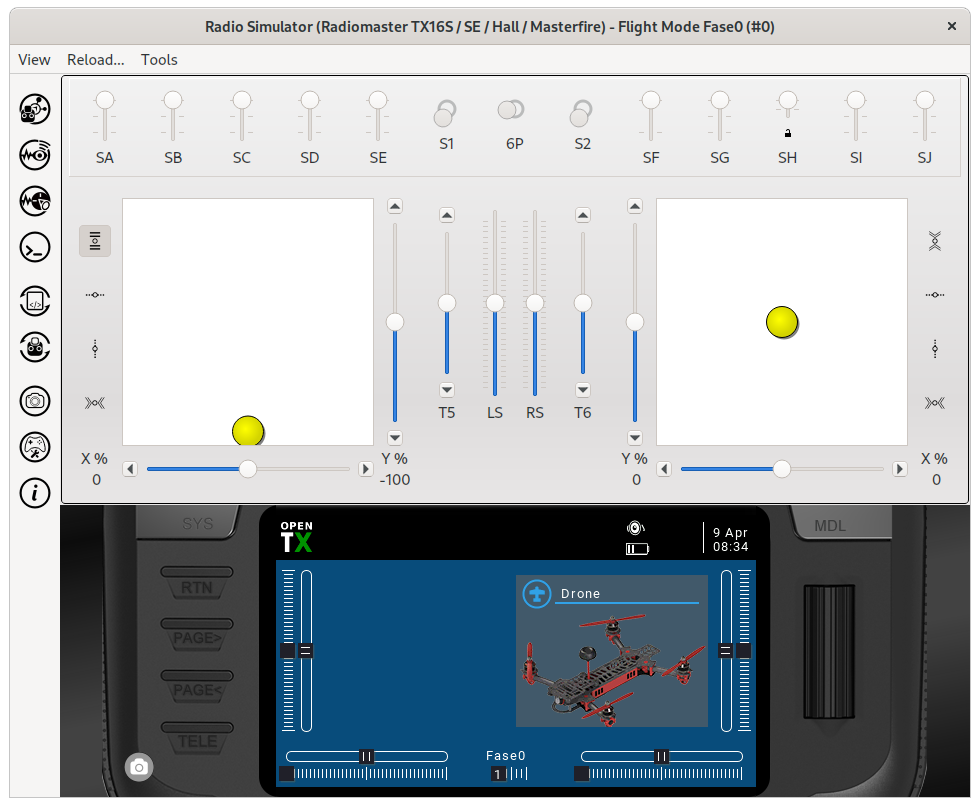
\includegraphics[ width=0.80\linewidth, height=\textheight, keepaspectratio]{./Pictures/opentx-sim-first.png}
        \caption{Simulazione del radiocomando \emph{RadioMaster TX16S} in OpenTX Simulator.}
        \label{fig:opentx-sim-first}
\end{figure}

\begin{figure}[ht]
        \centering
        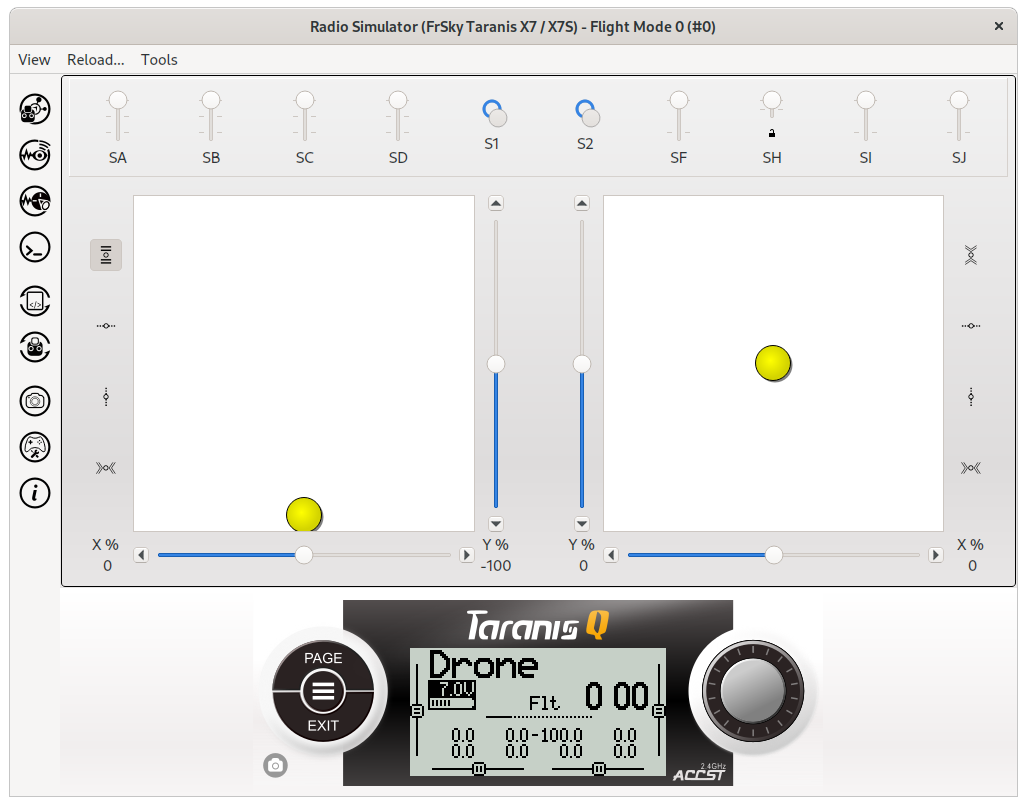
\includegraphics[ width=0.80\linewidth, height=\textheight, keepaspectratio]{./Pictures/opentx-sim-qx7s.png}
        \caption{Simulazione del radiocomando \emph{Taranis FrSky QX7S} in OpenTX Simulator.}
        \label{fig:opentx-sim-qx7s}
\end{figure}

Degna di nota è la schermata di configurazione dei modelli. Per ciascuno di esso infatti, navigando sul nome del modello, tasto destro del mouse, ``Edit Model'', è possibile accedere alla configurazione avanzata. È possibile impostare:
\begin{itemize}
        \item   i \emph{timer}, sistemi di radio interni ed esterni, il \emph{trainer}, nome ed immagine di modello;
        \item   le \emph{modalità di volo};
        \item   gli \emph{input}, i \emph{mixer} e gli \emph{output};
        \item   le \emph{curve};
        \item   i \emph{logical switches}, interruttori logici utilizzati per comparare valori e combinare il verificarsi di varie condizioni;
        \item   le \emph{special functions}, per la riproduzione di annunci personalizzati, attivazione della modalità trainer e così via;
        \item   la \emph{telemetria}.
\end{itemize}

Per l'avvio e l'utilizzo degli script trattati in questo elaborato si è resa necessaria la configurazione della telemetria di entrambi i radiocomandi adottati. Per il \emph{Taranis FrSky QX7S} sono state configurate due schermate di telemetria, una per ciascuno dei due script Lua. Nel caso del \emph{RadioMaster TX16S}, invece, si è fatto uso della configurazione dei widget direttamente dall'interfaccia del radiocomando in fase di simulazione, pertanto non è stato necessario adoperare il programma Companion per l'aggiunta delle interfacce di telemetria.

Il vantaggio legato all'utilizzo di OpenTX Companion è stato quello di poter configurare il radiocomando mediante interfaccia grafica su un sistema operativo per computer desktop. Inoltre, di fondamentale importanza è stata la facoltà di poter personalizzare e simulare i radiocomandi senza richiedere la loro presenza in ogni fase del progetto.

\clearpage

\chapter{RISULTATI E DISCUSSIONE}
In questo elaborato di tesi sperimentale sono stati realizzati due script Lua, lo \emph{script di cronometro vocale} (\texttt{TmrCnt}) e lo \emph{script di conto alla rovescia vocale} (\texttt{CntDwn}), ciascuno dei quali è stato realizzato per ambedue i modelli di radiocomando adoperati, il \emph{Taranis FrSky QX7S} ed il \emph{RadioMaster TX16S}.

\section{Lo script di cronometro vocale}\label{sec:tmrcnt}
L'obiettivo dello \emph{script di cronometro vocale} è stato quello di fornire al pilota in tempo reale un'indicazione sia visiva che acustica del tempo trascorso dall'inizio della fase di volo. Le informazioni del cronometro, oltre che visualizzate sull'apposita schermata di telemetria, sono riprodotte dal radiocomando come annunci vocali, consentendo di mantenere un maggiore controllo del tempo totale di volo senza la necessità di interrompere il contatto visivo con il drone per la visualizzazione dell'informazione sul display del radiocomando.

Lo script legge il tempo da un timer a scelta fra quelli messi a disposizione dal radiocomando, e consente di impostare un \emph{tempo di allarme} (\texttt{Alert}) in secondi. Esso rappresenta l'intervallo di tempo che intercorre fra un annuncio vocale ed il seguente. Quando il timer raggiunge un valore in secondi multiplo del tempo di allarme, viene riprodotto un annuncio vocale che comunica il tempo attualmente trascorso dall'avvio del timer.

Lo script di cronometro vocale fa ampiamente uso delle funzioni \texttt{lcd} in precedenza presentate nella sezione~\ref{section:funzioni-lcd} per sfruttare al meglio le capacità offerte dagli schermi dei due modelli.

\subsection{Widget \texttt{TmrCnt} su RadioMaster TX16S}

Lo script è il file \texttt{/WIDGETS/TmrCnt/main.lua}.

La parte iniziale dello script è composta dalle variabili locali, dalla table \texttt{options}, e dalle funzioni \texttt{create()} e \texttt{update()}:

\begin{lstlisting}
local played = false

local options = {
        { "Color", COLOR, BLUE }, 
        { "Timer", VALUE, 1, 1, 3 }, -- Timer 1, 2 o 3
        { "Alert", VALUE, 30, 15, 180 } -- Numero di secondi fra ciascun annuncio
}

local function create (zone, options)
        local widget = { zone=zone, options=options }
        return widget
end

local function update(widget, options)
        if (widget ~= nil) then
                widget.options = options
        end
end
\end{lstlisting}

Ad eccezione della table \texttt{options}, l'unica variabile locale dello script è il flag di controllo per la riproduzione \texttt{played}, inizialmente con valore \texttt{false}.

Nella table delle opzioni sono contenuti tre elementi: \texttt{\{ "Color", COLOR, BLUE \}} che permette di impostare il colore del testo desiderato, \texttt{\{ "Timer", VALUE, 1, 1, 3 \}} che consente la selezione del timer del radiocomando e \texttt{\{ "Alert", VALUE, 30, 15, 180 \}} grazie al quale è possibile assegnare un intervallo personalizzato di secondi fra un annuncio ed il seguente ed il cui valore predefinito è $30$.

Successivamente alle variabili dello script sono definite le funzioni \texttt{create()} ed \texttt{update()}. Esse si occupano, rispettivamente, di generare il widget e di aggiornare le opzioni successivamente alle modifiche effettuate dall'utente.

Altrettanto necessarie al funzionamento del widget sono le funzioni \texttt{refresh()} e\newline \texttt{background()}, con le elaborazioni opportunamente suddivise nelle funzioni \texttt{playTimer()} e \texttt{drawByWidgetSize()} le quali, rispettivamente, hanno il compito di gestire l'esecuzione degli annunci vocali e della stampa su schermo:

\begin{lstlisting}
local function refresh(widget)
        local timer = model.getTimer(widget.options.Timer - 1)
        drawByWidgetSize(widget, timer)
        playTimer(timer, widget.options.Alert)
end
local function background(widget)
        local timer = model.getTimer(widget.options.Timer - 1)
        playTimer(timer, widget.options.Alert)
end
\end{lstlisting}

Sia la funzione \texttt{background()} che \texttt{refresh()} eseguono la funzione \texttt{playTimer()}. Viene qua riportata:

\begin{lstlisting}
local function playTimer(timer, alert)
        if timer.value % alert == 1 then
                played = false
        end
        if  timer.value % alert == 0 and timer.value ~= 0 then
                if played == false then
                        playDuration(timer.value, 0)
                        played = true
                end
        end
end 
\end{lstlisting}

La funzione \texttt{playTimer()} riceve come argomenti un timer e il valore \texttt{alert}, a cui viene passato il valore \texttt{Alert} delle opzioni. Se il valore in secondi del timer è un multiplo di \texttt{alert} e contemporaneamente non è pari a $0$, viene riprodotto l'annuncio vocale ed il flag \texttt{played} assume il valore \texttt{true}. Nelle iterazioni successive il flag impedisce all'annuncio vocale di essere riprodotto nuovamente: esso verrà ripristinato al valore \texttt{false} soltanto quando il timer passa al secondo successivo, in condizioni nelle quali l'annuncio non può più essere riprodotto. In assenza di un flag di controllo, l'annuncio vocale verrebbe riprodotto ad ogni nuova iterazione della funzione \texttt{refresh()} o \texttt{background()}, ottenendo la ripetizione indesiderata dell'annuncio vocale.

Le funzioni di stampa su schermo sono interamente contenute all'interno della funzione \newline\texttt{drawBywidgetSize()}, la quale accetta come argomenti un widget ed un timer. Inizialmente è estratto il numero del timer nel formato \texttt{T\%s}, ed il colore scelto nelle opzioni dello script viene assegnato agli elementi dello script quali testo e numeri mediante il metodo \texttt{lcd.setColor()}, indicando come primo argomento \texttt{CUSTOM\_COLOR}: 

\begin{lstlisting}
local function drawByWidgetSize(widget, timer)
        local timerInfo = string.format("T%s:", widget.options.Timer)
        lcd.setColor(CUSTOM_COLOR, widget.options.Color)
\end{lstlisting}

Per la stampa vera e propria si adoperano i metodi \texttt{lcd.drawText()} ed \texttt{lcd.drawTimer()}. Ad essi vengono passati come argomenti la posizione orizzontale e verticale relativamente all'angolo in alto a sinistra del widget (avente coordinate \texttt{widget.zone.x} e \texttt{widget.zone.y}), l'informazione da stampare su schermo e flag relativi alla dimensione del testo e al colore. Questa sezione è stata realizzata in modo tale da distinguere le possibili dimensioni del widget supportate dal \emph{RadioMaster TX16S} mediante delle istruzioni \texttt{if} che valutano la larghezza del widget (contenuta nella variabile \texttt{widget.zone.w}) e la sua altezza (contenuta in \texttt{widget.zone.h}). Vi sono in totale $5$ diverse dimensioni per i widget del \emph{RadioMaster TX16S}, ottenute empiricamente. In particolare:

\begin{itemize}
        \item \emph{widget molto grande}: per larghezze maggiori di $380$ pixel e altezze maggiori di $165$ pixel;
        \item \emph{widget grande}: per larghezze maggiori di $180$ pixel e altezze maggiori di $145$ pixel;
        \item \emph{widget medio}: per larghezze maggiori di $170$ pixel e altezze maggiori di $65$ pixel;
        \item \emph{widget piccolo}: per larghezze maggiori di $150$ pixel e altezze maggiori di $28$ pixel;
        \item \emph{widget nella barra superiore}: per larghezze maggiori di $65$ pixel e altezze maggiori di $35$ pixel.
\end{itemize}

Ad esempio, al \emph{widget molto grande} corrisponde la seguente istruzione \texttt{if}:

\begin{lstlisting}
        -- Widget a schermo intero
        if widget.zone.w > 380 and widget.zone.h > 165 then
                lcd.drawText(widget.zone.x, widget.zone.y, timerInfo, DBLSIZE + CUSTOM_COLOR)
                lcd.drawTimer(widget.zone.x + 100, widget.zone.y + 40, timer.value, XXLSIZE + CUSTOM_COLOR)
        end
\end{lstlisting}

e similmente vi saranno ulteriori \texttt{if} per tutte le altre dimensioni supportate.

Gli offset della posizione orizzontale e verticale dei vari elementi del widget, così come le dimensioni del testo, sono stati anch'essi determinati empiricamente, valutando la leggibilità e la corretta posizione mediante dei tentativi effettuati all'interno del simulatore \emph{OpenTX Simulator}.

Al termine dello script, è collocato lo statement di \texttt{return}:

\begin{lstlisting}
return { name="TmrCnt", options=options, create=create, update=update, background=background, refresh=refresh }
\end{lstlisting}

La Figura~\ref{fig:tmrcnt-tx16s} mostra l'aspetto dello script durante la sua esecuzione.

\begin{figure}[ht]
        \centering
        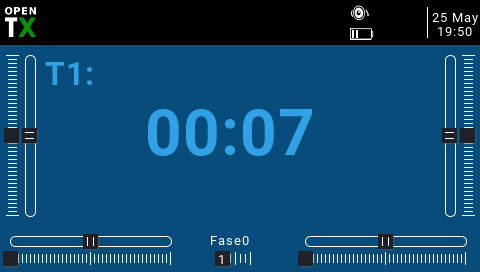
\includegraphics[ width=0.70\linewidth, height=\textheight, keepaspectratio]{./Pictures/tmrcnt-tx16s.png}
        \caption{Aspetto della schermata del \emph{RadioMaster TX16S} durante l'esecuzione dello script \texttt{TmrCnt}. La dimensione del widget è la massima disponibile.}
        \label{fig:tmrcnt-tx16s}
\end{figure}


\subsection{Schermata di telemetria \texttt{TmrCnt} su Taranis QX7S}

Lo script è il file \texttt{/SCRIPTS/TELEMETRY/TmrCnt.lua}.

Diversamente da quanto visto in precedenza per il \emph{TX16S}, il \emph{Taranis QX7S} non supporta i widget e pertanto non fornisce la possibilità di impostare le variabili mediante le opzioni direttamente da radiocomando. Al fine di garantire un'analoga capacità di personalizzazione, sono rese disponibili alcune variabili di configurazione all'inizio dello script, modificabili mediante un editor di testo:

\begin{lstlisting}
local TimerNumber = 1
local Alert = 30                
local InversColor = false
\end{lstlisting}

\texttt{TimerNumber} permette la selezione del timer del radiocomando, con possibili valori $1$, $2$ e $3$, mentre l'opzione \texttt{"Alert"} presente nella versione per il \emph{TX16S} è stata sostituita dalla variabile \texttt{Alert}. La variabile booleana \texttt{InversColor}, invece, consente di abilitare l'inversione dei colori su schermo.

Successivamente a tale sezione sono collocate le variabili interne dello script, la cui modifica da parte dell'utente non è prevista poiché potrebbe alterare il funzionamento dello script. Le variabili sono \texttt{Timer}, che contiene il timer, \texttt{TimerInfo} che contiene la stringa identificativa del timer e il flag \texttt{Played}:

\begin{lstlisting}
local Timer
local TimerInfo
local Played 
\end{lstlisting}

Le funzioni principali, \texttt{init()}, \texttt{run()} e \texttt{background()} si occupano, rispettivamente, della configurazione iniziale, della stampa su schermo quando la schermata è visibile, e della riproduzione degli annunci a prescindere dalla visibilità della schermata.

\begin{lstlisting}
local function init()
        Timer = model.getTimer(TimerNumber - 1)
        TimerInfo = string.format("T%s:", TimerNumber)
        Played = false
end

local function refresh()
        drawTelemetry()
end

local function background()
        Timer = model.getTimer(TimerNumber - 1)
        playTimer()
end
\end{lstlisting}

Le elaborazioni interne sono ancora una volta suddivise in ulteriori funzioni. La funzione \texttt{playTimer()} è del tutto analoga a quella per il \emph{TX16S}, e presenta il medesimo algoritmo con flag \texttt{Played} per il controllo della riproduzione degli annunci vocali.

In particolare:

\begin{lstlisting}
local function playTimer()
        if Timer.value % Alert == 1 then
                Played = false
        end

        if  Timer.value % Alert == 0 and Timer.value ~= 0 then
                if Played == false then
                        playDuration(Timer.value, 0)
                        Played = true
                end
        end
end 
\end{lstlisting}

La stampa su schermo è invece differente, sia poiché è assente il concetto di widget con le varie dimensioni supportate, sia per la presenza di alcune funzioni indispensabili al funzionamento degli script di Telemetria. 

\begin{lstlisting}
local function drawTelemetry()
        lcd.clear() -- obbligatorio negli script di Telemetria
        lcd.drawScreenTitle("Timer Counter", 0, 0)
        if InversColor == true then
                lcd.drawFilledRectangle(0, 0, 128, 64)
                lcd.drawText(0, 9, TimerInfo, INVERS)
                lcd.drawTimer(13, 18, Timer.value, XXLSIZE + INVERS)
        else
                lcd.drawText(0, 9, TimerInfo, BIGSIZE)
                lcd.drawTimer(13, 18, Timer.value, XXLSIZE)
        end
end
\end{lstlisting}

Un'istruzione \texttt{if} consente inoltre di determinare se l'utente desidera una stampa a colori invertiti: in tal caso, viene stampato su schermo un opportuno rettangolo di colore scuro, e agli stessi comandi è aggiunto il flag \texttt{INVERS} in modo tale da riprodurre le stringhe con caratteri chiari su sfondo scuro.

L'istruzione di return è collocata alla fine dello script:

\begin{lstlisting}
return { run=refresh, background=background, init=init }
\end{lstlisting}

L'aspetto originale e la versione a colori invertiti sono mostrati, rispettivamente, in Figura~\ref{fig:tmrcnt-qx7s} ed in Figura~\ref{fig:tmrcnt-qx7s-i}.

\begin{figure}[ht]
        \centering
        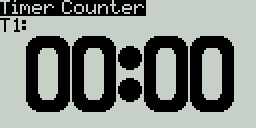
\includegraphics[ width=0.70\linewidth, height=\textheight, keepaspectratio]{./Pictures/tmrcnt-qx7s.png}
        \caption{Aspetto della schermata di telemetria del \emph{Taranis QX7S} durante l'esecuzione dello script \texttt{TmrCnt}.}
        \label{fig:tmrcnt-qx7s}
\end{figure}

\begin{figure}[ht]
        \centering
        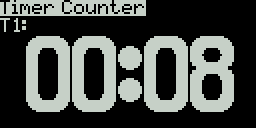
\includegraphics[ width=0.70\linewidth, height=\textheight, keepaspectratio]{./Pictures/tmrcnt-qx7s-i.png}
        \caption{Aspetto a colori invertiti della schermata di telemetria del \emph{Taranis QX7S} durante l'esecuzione dello script \texttt{TmrCnt}.}
        \label{fig:tmrcnt-qx7s-i}
\end{figure}

\section{Lo script di conto alla rovescia vocale}
L'obiettivo dello \emph{script di conto alla rovescia vocale} è stato quello di fornire un conto alla rovescia personalizzabile, garantendo al pilota in tempo reale un'indicazione acustica del tempo residuo. Le informazioni del conto alla rovescia sono riprodotte dal radiocomando come annunci vocali, consentendo di mantenere un maggiore controllo del tempo rimanente senza la necessità di interrompere il contatto visivo con il drone per la visualizzazione dell'informazione sul display del radiocomando.

Lo script legge il tempo da un timer del radiocomando, e consente di impostare un \emph{tempo di partenza} (\texttt{Start}) in secondi. Esso rappresenta il numero iniziale di secondi del conto alla rovescia. Quando il timer raggiunge un multiplo del minuto, o un sottomultiplo del minuto se il tempo rimanente è inferiore a $60$ secondi, viene riprodotto un annuncio vocale contenente il tempo residuo.

Lo script di conto alla rovescia vocale fa ampiamente uso delle funzioni \texttt{lcd} in precedenza presentate nella sezione~\ref{section:funzioni-lcd} per sfruttare al meglio le capacità offerte dagli schermi dei due modelli.



\subsection{Widget \texttt{CntDwn} su RadioMaster TX16S}

Lo script è il file \texttt{/WIDGETS/CntDwn/main.lua}.

La parte iniziale dello script è composta dalla definizione delle opzioni, dalla dichiarazione di alcune variabili locali e dalle funzioni \texttt{create()} ed \texttt{update()}:

\begin{lstlisting}
local options = {
        { "Color", COLOR, BLUE },
        { "Timer", VALUE, 1, 1, 3 },
        { "Start", VALUE, 180, 30, 600 }
}

local Total             -- numero totale di secondi
local NextSecond = 11   -- variabile di controllo per gli ultimi 10 secondi
local Played            -- flag di controllo
local Elapsed           -- flag che controlla il termine del conto alla rovescia

local function create (zone, options)
        local widget = { zone=zone, options=options }
        Total = widget.options.Start
        Played = false
        Elapsed = false
        return widget
end

local function update(widget, options)
        if (widget ~= nil) then
                widget.options = options
        end
        Total = widget.options.Start
        Played = false
        Elapsed = false
end
\end{lstlisting}

La struttura ricalca quella dello script \texttt{TmrCnt}, e differenze degne di nota sono la presenza del valore di inizio del cronometro, nelle opzioni \texttt{"Start"}, e la presenza di più flag, con aggiornamento dei flag \texttt{Played} ed \texttt{Elapsed} all'interno della funzione \texttt{update()} per riportare il cronometro alle nuove condizioni iniziali al momento della modifica delle opzioni da parte del pilota.

All'interno delle due funzioni principali, \texttt{refresh()} e \texttt{background()}, viene calcolato il numero di secondi rimanente allo scadere del conto alla rovescia, \texttt{countdown}, e successivamente tale valore è stampato su schermo nel caso della funzione \texttt{refresh()} e riprodotto acusticamente nel caso di ambedue le funzioni.

Si osserva che le due funzioni svolgono le stesse elaborazioni, eccezion fatta per l'assenza di interazione con lo schermo nella funzione \texttt{background()}:

\begin{lstlisting}
local function refresh(widget)
        local timer = model.getTimer(widget.options.Timer - 1)
        local countdown

        if Total - timer.value > 0 then
                countdown = Total - timer.value
        else
                countdown = 0
        end

        drawByWidgetSize(widget, countdown)

        if Elapsed == false then
                playTime(countdown)
        end
end


local function background(widget)
        local timer = model.getTimer(widget.options.Timer - 1)
        local countdown

        if Total - timer.value > 0 then
                countdown = Total - timer.value
        else
                countdown = 0
        end

        if Elapsed == false then
                playTime(countdown)
        end
end
\end{lstlisting}

La funzione di stampa su schermo ha funzioni analoghe a quanto osservato per lo script \texttt{TmrCnt}: la dimensione e la posizione del testo viene selezionata in base alle dimensioni del widget, e successivamente si utilizza la funzione \texttt{lcd.drawNumber()} con gli opportuni argomenti per la stampa del contatore il cui valore è contenuto nella variabile \texttt{countdown}.

Differenze sostanziali si trovano nella riproduzione degli annunci vocali. È stato scelto di riprodurre annunci ogni $60$ secondi, mentre durante l'ultimo minuto viene comunicato un avviso ai secondi $30$, $15$, $10$, $9$, $8$, $7$, $6$, $5$, $4$, $3$, $2$, $1$. Allo scadere del conto alla rovescia viene riprodotto l'annuncio finale.

L'utilizzo del flag \texttt{Played} ha consentito ancora una volta di evitare le riproduzioni multiple che si sarebbero altrimenti verificate. 

Allo scadere del tempo, il flag \texttt{Elapsed} al valore \texttt{true} impedisce la chiamata alla funzione \texttt{playTime()}, prevenendo elaborazioni superflue.

Viene riportata la funzione:

\begin{lstlisting}
local function playTime(countdown)

        local seconds = countdown % 60 
        local minutes = (countdown - seconds) / 60

        if Played == true then
                resetPlayedFlag(countdown, NextSecond)
        end

        if Played == false then
                if countdown > 30 then
                        if countdown % 60 == 0 and countdown ~= Total then
                                if minutes ~= 0 and seconds == 0 then
                                        playNumber(minutes, 36)
                                else
                                        playNumber(minutes, 36)
                                        playNumber(seconds, 37)
                                end
                                Played = true
                        end
                elseif countdown == 30 then
                        playNumber(countdown, 37)
                        Played = true
                elseif countdown == 15 then
                        playNumber(countdown, 37)
                        Played = true
                elseif countdown <= 10 and countdown > 0 then
                        playNumber(countdown, UNIT_RAW)
                        Played = true
                        NextSecond = countdown
                elseif countdown == 0 then
                        playFile("/WIDGETS/Cntdwn/timelpsd.wav")
                        Played = true
                        Elapsed = true
                end
        end
end
\end{lstlisting}

A causa della maggiore complessità nel determinare le condizioni per il ripristino del flag \texttt{Played} al valore \texttt{false}, tale compito è affidato ad un'ulteriore funzione, \texttt{resetPlayedFlag()}, la quale si occupa di stabilire le condizioni opportune per la modifica del flag:

\begin{lstlisting}
local function resetPlayedFlag(countdown, NextSecond)
        if countdown % 60 == 59 then
                Played = false
        elseif countdown == 29 or countdown == 14 then
                Played = false
        elseif countdown <= 10 and Elapsed ~= true and countdown ~= NextSecond then
                Played = false
        end
end
\end{lstlisting}

La variabile \texttt{NextSecond} consente di stabilire, per gli ultimi $10$ secondi, un criterio per la reimpostazione del flag \texttt{Played} al valore \texttt{false}. Infatti, \texttt{NextSecond} conterrà il valore di \texttt{countdown} negli ultimi $10$ secondi, ed il ripristino del flag ha luogo soltanto se queste due variabili hanno valore differente, condizione che può verificarsi solo immediatamente dopo il decremento di \texttt{countdown}.


Lo script si presenta come in Figura~\ref{fig:cntdwn-tx16s}.

\begin{figure}[ht]
        \centering
        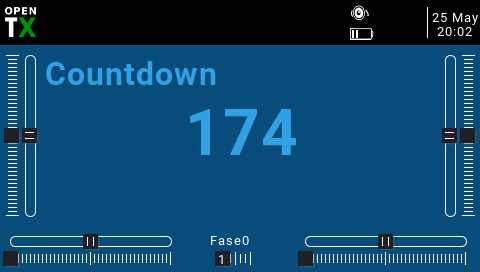
\includegraphics[ width=0.70\linewidth, height=\textheight, keepaspectratio]{./Pictures/cntdwn-tx16s.png}
        \caption{Aspetto della schermata del \emph{RadioMaster TX16S} durante l'esecuzione dello script \texttt{CntDwn}. La dimensione del widget è la massima disponibile.}
        \label{fig:cntdwn-tx16s}
\end{figure}

\subsection{Schermata di telemetria \texttt{CntDwn} su Taranis QX7S}

La struttura per lo script di conto alla rovescia vocale nel \emph{QX7S} presenta poche differenze rispetto alla versione per il \emph{TX16S}. 

In sostituzione delle opzioni è fornita una sezione dello script contenente le variabili di configurazione, per cui è possibile configurarne manualmente il valore mediante un editor di testo. Esse sono il numero del timer \texttt{TimerNumber}, il totale dei secondi del conto alla rovescia\newline \texttt{CountdownTotalSeconds} e l'inversione dei colori \texttt{InversColor}:

\begin{lstlisting}
local TimerNumber = 1
local CountdownTotalSeconds = 180
local InversColor = false
\end{lstlisting}

Le variabili interne dello script sono dichiarate nella sezione immediatamente successiva, e fra di esse, oltre alle medesime variabili della versione per il \emph{TX16S}, troviamo \texttt{Timer} e \texttt{TimerInfo} che conterranno, rispettivamente, il timer del radiocomando e le relative informazioni.

La gestione della riproduzione degli annunci non presenta nessuna variazione degna di nota rispetto alla versione per il \emph{TX16S}: ancora una volta l'elaborazione è stata suddivisa nelle due funzioni \texttt{playTime()} e \texttt{resetPlayedFlag()} le quali svolgono le stesse computazioni della variante per il \emph{RadioMaster}.

Come già osservato per lo script \texttt{TmrCnt}, a presentare alcune differenze è la funzione di stampa su schermo, che in questa variante prende il nome di \texttt{drawTelemetry()}. Nuovamente sono assenti il concetto di widget ed i relativi \texttt{if} necessari all'identificazione della dimensione correntemente selezionata dall'utente nell'interfaccia del radiocomando: al loro posto vi è la stampa delle informazioni e la possibilità di invertire i colori modificando il valore della variabile di configurazione \texttt{InversColor},

\begin{lstlisting}
local function drawTelemetry()
        lcd.clear() 
        lcd.drawScreenTitle("Countdown Timer", 0, 0)
        if InversColor == true then
                lcd.drawFilledRectangle(0, 0, 128, 64)
                lcd.drawText(0, 9, TimerInfo, INVERS)
                lcd.drawNumber(3, 18, Countdown, XXLSIZE + INVERS)
        else
                lcd.drawText(0, 9, TimerInfo, BIGSIZE)
                lcd.drawNumber(3, 18, Countdown, XXLSIZE)
        end
end
\end{lstlisting}

Le due funzioni principali, \texttt{refresh()} e \texttt{background()} svolgono le medesime elaborazioni della variante per il \emph{TX16S}.

L'aspetto originale e la versione a colori invertiti sono mostrati, rispettivamente, in Figura~\ref{fig:cntdwn-qx7s} ed in Figura~\ref{fig:cntdwn-qx7s-i}.

\begin{figure}[ht]
        \centering
        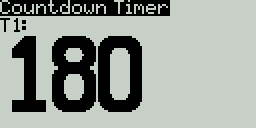
\includegraphics[ width=0.70\linewidth, height=\textheight, keepaspectratio]{./Pictures/cntdwn-qx7s.png}
        \caption{Aspetto della schermata di telemetria del \emph{Taranis QX7S} durante l'esecuzione dello script \texttt{CntDwn}.}
        \label{fig:cntdwn-qx7s}
\end{figure}

\begin{figure}[ht]
        \centering
        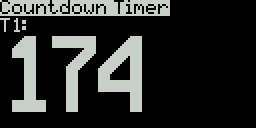
\includegraphics[ width=0.70\linewidth, height=\textheight, keepaspectratio]{./Pictures/cntdwn-qx7s-i.png}
        \caption{Aspetto a colori invertiti della schermata di telemetria del \emph{Taranis QX7S} durante l'esecuzione dello script \texttt{CntDwn}.}
        \label{fig:cntdwn-qx7s-i}
\end{figure}



\clearpage



\chapter{CONCLUSIONI}

OpenTX mette a disposizione agli sviluppatori software vari strumenti e applicativi di notevole utilità. Lo studio della documentazione, l'apprendimento di \emph{OpenTX Companion} e la fase di test dei due script, avvenuta integralmente tramite il simulatore \emph{OpenTX Simulator}, ha infine portato alla realizzazione di due script di telemetria, in grado di svolgere compiti ed elaborazioni personalizzate. 

L'integrazione con il linguaggio di scripting Lua consente allo sviluppatore di potenziare ulteriormente le già ampie possibilità offerte dal firmware all'interno del radiocomando, in particolare dotando i vari modelli di trasmittente di ampie capacità di calcolo e di elaborazione.

La documentazione del progetto, esauriente ed aggiornata, ha permesso uno studio approfondito e dettagliato della materia, con particolare attenzione alla parte relativa al supporto degli script in Lua.

Il software principale per computer desktop, \emph{OpenTX Companion}, ha reso possibile la gestione avanzata e da interfaccia grafica delle impostazioni del radiocomando, della loro personalizzazione e del loro salvataggio anche in assenza di un radiocomando reale. Il secondo programma, il simulatore, ha poi consentito il test delle impostazioni stesse del radiocomando e, con sufficiente realismo, anche degli script in Lua realizzati in questo elaborato di tesi sperimentale.

Al termine della loro stesura e sperimentazione mediante il simulatore, i programmi sono stati sperimentati dal vivo sui due radiocomandi reali, il \emph{Taranis QX7S} ed il \emph{RadioMaster TX16S}. La prova ha dato esito positivo per ambedue gli script, su entrambi i modelli, e sia lo script di cronometro vocale (\texttt{TmrCnt}) che lo script di conto alla rovescia (\texttt{CntDwn}) hanno manifestato un comportamento idoneo e nel pieno rispetto di quanto era stato inizialmente progettato e testato nel simulatore. Il risultato ha risposto alle aspettative, ed è stato dunque del tutto soddisfacente.


\chapter{SVILUPPI FUTURI}

Gli sviluppi futuri potrebbero essere rivolti alla creazione di un maggiormente complesso sistema di telemetria. È infatti possibile ottenere ed elaborare ulteriori dati fra cui l'\emph{RSSI} (Received Signal Strength Indication), la lettura della tensione della batteria del radiocomando, la lettura della tensione della batteria del modello. In particolare, l'RSSI è ottenibile mediante la funzione \texttt{getRSSI()}, la quale restituirà un valore intero fra 0 e 99 che indica l'intensità del segnale in ricezione, mentre la lettura della tensione avviene prelevando il dato da una sorgente (\texttt{SOURCE}) come definita nella sezione~\ref{subsec:struttura-script-modello}. Il nome della sorgente può presentare variazioni a seconda del radiocomando o del modello adottato. Nei due radiocomandi in esame essa prende il nome di \texttt{tx-voltage}, mentre possibili nomi di sorgenti per la tensione di batteria del modello sono \texttt{RxBt} oppure \texttt{VFAS}. All'ottenimento della tensione del modello potrebbero seguire ulteriori elaborazioni, con particolare attenzione alle problematiche relative alla stima della batteria residua o all'individuazione di eventuali malfunzionamenti. 

D'importanza cruciale sarebbe la corretta gestione dei relativi annunci vocali, al fine di sollevare il pilota della responsabilità di mantenere un contatto visivo con lo schermo del radiocomando.

Uno sviluppo più avanzato porterebbe infine al progetto e alla gestione di un complesso sistema di telemetria che presenti coerentemente e su un'unica schermata tutti i dati necessari al pilota (cronometro vocale, tensioni di batterie, coordinate GPS, RSSI e così via), sia come numeri filtrati da opportune elaborazioni con relative stringhe di testo, che in qualità di annunci vocali.

\clearpage




%% Marco Sgobino
%% Tesi di laurea triennale
% file-bibliografia.tex
\titleformat{\chapter}[display]
{\Huge\bfseries}{}{0pt}{}
\clearpage
\addcontentsline{toc}{chapter}{Bibliografia}
\begin{thebibliography}{9}
        \bibitem{opentx-website} OpenTX, \underline{https://www.open-tx.org/}, 2014.
        \bibitem{opentx-radios} OpenTX, \underline{https://www.open-tx.org/radios}, 2014.
        \bibitem{opentx-github} Repository OpenTX su GitHub, \underline{https://github.com/opentx/opentx}, 2021.
        \bibitem{oss-osh-uavs} Burdziakowski, P., Razmjooy, N., Estrela, V., \& Hemanath, J. (2020). \emph{``Open-source software (OSS) and hardware (OSH) in UAVs''}. 49-66
        \bibitem{mission-planner-website} ArduPilot Dev Team, \underline{https://ardupilot.org/planner/}, 2021.
        \bibitem{ardupilot-website} ArduPilot, \underline{https://ardupilot.org/}, 2016.
        \bibitem{opendronemap} OpenDroneMap Authors ODM, \emph{``A command line toolkit to generate maps, point clouds, 3D models and DEMs from drone, balloon or kite images.''} \underline{https://github.com/OpenDroneMap/ODM}, 2020.
        \bibitem{webodm-website} UAV4GEO, \underline{https://webodm.net/}.
        \bibitem{rise-uavs} Cummings, Anthony R.; McKee, Arlo; Kulkarni, Keyur; Markandey, Nakul, \emph{``The Rise of UAVs''}, Photogrammetric Engineering \& Remote Sensing, Volume 83, Number 4, April 2017, pp. 317-325(9)
        \bibitem{italy-uavs} Andrea Cardamone, \emph{``Implementation of a pilot in the loop simulation environment for UAV development and testing''}, \underline{http://hdl.handle.net/10589/135202} 2017.
        \bibitem{opentx-firmware} OpenTXU, \underline{http://open-txu.org/home/undergraduate-courses/introduction/how-rc-works/}, 2014.
        \bibitem{opentx-lua-instructions} OpenTX, \underline{https://www.open-tx.org/lua-instructions.html}, 2014.
        \bibitem{lua-website} Lua Project, \underline{https://www.lua.org/}, 2020.
        \bibitem{opentx-companion-manual} OpenTX, \underline{https://doc.open-tx.org/manual-for-opentx-2-2/companion}.
        \bibitem{fedora-website} Fedora Project, \underline{https://getfedora.org/}, 2021.
        \bibitem{opentx-download-page} OpenTX, \underline{https://www.open-tx.org/downloads}, 2014.
\end{thebibliography}

% https://www.ingentaconnect.com/content/asprs/pers/2017/00000083/00000004/art00016#
% https://mostwiedzy.pl/pl/publication/open-source-software-oss-and-hardware-osh-in-uavs,152706-1
% https://www.politesi.polimi.it/handle/10589/135202?mode=complete

\addcontentsline{toc}{chapter}{Appendice}
\chapter*{Appendice}
\addcontentsline{toc}{section}{Script \texttt{TmrCnt} per RadioMaster TX16S}
\section*{Script \texttt{TmrCnt} per RadioMaster TX16S}

\begin{lstlisting}
-- Timer Counter Widget
-- Nome: TmrCnt
--
-- File: "main.lua"
-- Da collocare in "/WIDGETS/TmrCnt/"

local played = false

local options = {
        { "Color", COLOR, BLUE }, 
        { "Timer", VALUE, 1, 1, 3 }, -- Timer 1, 2 o 3
        { "Alert", VALUE, 30, 15, 180 } -- Numero di secondi fra ciascun annuncio
}

local function create (zone, options)
        local widget = { zone=zone, options=options }
        return widget
end

local function update(widget, options)
        if (widget ~= nil) then
                widget.options = options
        end
end

local function drawByWidgetSize(widget, timer)
        local timerInfo = string.format("T%s:", widget.options.Timer)
        lcd.setColor(CUSTOM_COLOR, widget.options.Color)

        -- Widget a schermo intero
        if widget.zone.w > 380 and widget.zone.h > 165 then
                lcd.drawText(widget.zone.x, widget.zone.y, timerInfo, DBLSIZE + CUSTOM_COLOR)
                lcd.drawTimer(widget.zone.x + 100, widget.zone.y + 40, timer.value, XXLSIZE + CUSTOM_COLOR)

        -- Widget Grande
        elseif widget.zone.w > 180 and widget.zone.h > 145 then
                lcd.drawText(widget.zone.x, widget.zone.y, timerInfo, MIDSIZE + CUSTOM_COLOR)
                lcd.drawTimer(widget.zone.x + 13, widget.zone.y + 25, timer.value, XXLSIZE + CUSTOM_COLOR)

        -- Widget Medio
        elseif widget.zone.w > 170 and widget.zone.h > 65 then
                lcd.drawText(widget.zone.x, widget.zone.y, timerInfo, SMLSIZE + CUSTOM_COLOR)
                lcd.drawTimer(widget.zone.x + 3, widget.zone.y + 5, timer.value, XXLSIZE + CUSTOM_COLOR)

        --Widget Piccolo
        elseif  widget.zone.w > 150 and widget.zone.h > 28 then
                lcd.drawText(widget.zone.x, widget.zone.y + 7, timerInfo, SMLSIZE + CUSTOM_COLOR)
                lcd.drawTimer(widget.zone.x + 70, widget.zone.y + 1, timer.value, MIDSIZE + CUSTOM_COLOR)

        -- Widget nella barra superiore
        elseif widget.zone.w > 65 and widget.zone.h > 35 then
                lcd.drawText(widget.zone.x, widget.zone.y, timerInfo, SMLSIZE + CUSTOM_COLOR)
                lcd.drawTimer(widget.zone.x, widget.zone.y + 10, timer.value, MIDSIZE + CUSTOM_COLOR)
        else
                lcd.drawText(widget.zone.x, widget.zone.y, "Insufficient space", SMLSIZE + CUSTOM_COLOR)
        end
end
        
local function playTimer(timer, alert)
        if timer.value % alert == 1 then
                played = false
        end

        if  timer.value % alert == 0 and timer.value ~= 0 then
                if played == false then
                        playDuration(timer.value, 0)
                        played = true
                end
        end
end 

local function refresh(widget)
        local timer = model.getTimer(widget.options.Timer - 1)
        drawByWidgetSize(widget, timer)
        playTimer(timer, widget.options.Alert)
end

local function background(widget)
        local timer = model.getTimer(widget.options.Timer - 1)
        playTimer(timer, widget.options.Alert)
end

return { name="TmrCnt", options=options, create=create, update=update, background=background, refresh=refresh }
\end{lstlisting}

\clearpage

\addcontentsline{toc}{section}{Script \texttt{TmrCnt} per Taranis QX7S}
\section*{Script \texttt{TmrCnt} per Taranis QX7S}
\begin{lstlisting}
-- File TmrCnt.lua
--
-- Script "Timer Counter"
--
-- Da collocare in "/SCRIPTS/TELEMETRY/"
--
-- impostazioni e variabili modificabili 
local TimerNumber = 1
local Alert = 30                
local InversColor = false

-- variabili di script 
-- Non modificare al di sotto di questa riga
local Timer
local TimerInfo
local Played 

-- funzioni dello script 
local function playTimer()
        if Timer.value % Alert == 1 then
                Played = false
        end

        if  Timer.value % Alert == 0 and Timer.value ~= 0 then
                if Played == false then
                        playDuration(Timer.value, 0)
                        Played = true
                end
        end
end 

local function drawTelemetry()
        lcd.clear() 
        lcd.drawScreenTitle("Timer Counter", 0, 0)
        if InversColor == true then
                lcd.drawFilledRectangle(0, 0, 128, 64)
                lcd.drawText(0, 9, TimerInfo, INVERS)
                lcd.drawTimer(13, 18, Timer.value, XXLSIZE + INVERS)
        else
                lcd.drawText(0, 9, TimerInfo, BIGSIZE)
                lcd.drawTimer(13, 18, Timer.value, XXLSIZE)
        end
end

-- funzioni principali 
local function init()
        Timer = model.getTimer(TimerNumber - 1)
        TimerInfo = string.format("T%s:", TimerNumber)
        Played = false
end

local function refresh()
        drawTelemetry()
end

local function background()
        Timer = model.getTimer(TimerNumber - 1)
        playTimer()
end

-- istruzione di return 
return { run=refresh, background=background, init=init }
\end{lstlisting}

\clearpage

\addcontentsline{toc}{section}{Script \texttt{CntDwn} per RadioMaster TX16S}
\section*{Script \texttt{CntDwn} per RadioMaster TX16S}
\begin{lstlisting}
-- File main.lua
-- Script "Countdown Timer"
--
-- Nome: "Cntdwn"
-- Da collocare in "/WIDGETS/Cntdwn/"

local options = {
        { "Color", COLOR, BLUE },
        { "Timer", VALUE, 1, 1, 3 },
        { "Start", VALUE, 180, 30, 600 }
}

local Total             
local NextSecond = 11   
local Played            
local Elapsed           

local function create (zone, options)
        local widget = { zone=zone, options=options }
        Total = widget.options.Start
        Played = false
        Elapsed = false
        return widget
end

local function update(widget, options)
        if (widget ~= nil) then
                widget.options = options
        end
        Total = widget.options.Start
        Played = false
        Elapsed = false
end

local function drawByWidgetSize(widget, countdown)
        lcd.setColor(CUSTOM_COLOR, widget.options.Color)

        -- Widget a schermo intero
        if widget.zone.w > 380 and widget.zone.h > 165 then
                lcd.drawText(widget.zone.x, widget.zone.y, "Countdown", DBLSIZE + CUSTOM_COLOR)
                lcd.drawNumber(widget.zone.x + 140, widget.zone.y + 40, countdown, XXLSIZE + CUSTOM_COLOR)

        -- Widget Grande
        elseif widget.zone.w > 180 and widget.zone.h > 145 then
                lcd.drawText(widget.zone.x, widget.zone.y, "Countdown", MIDSIZE + CUSTOM_COLOR)
                lcd.drawNumber(widget.zone.x + 13, widget.zone.y + 25, countdown, XXLSIZE + CUSTOM_COLOR)

        -- Widget Medio
        elseif widget.zone.w > 170 and widget.zone.h > 65 then
                lcd.drawText(widget.zone.x, widget.zone.y, "Countdown", SMLSIZE + CUSTOM_COLOR)
                lcd.drawNumber(widget.zone.x + 3, widget.zone.y + 5, countdown, XXLSIZE + CUSTOM_COLOR)

        -- Widget Piccolo
        elseif  widget.zone.w > 150 and widget.zone.h > 28 then
                lcd.drawText(widget.zone.x, widget.zone.y + 7, "Countdown", SMLSIZE + CUSTOM_COLOR)
                lcd.drawNumber(widget.zone.x + 90, widget.zone.y + 1, countdown, MIDSIZE + CUSTOM_COLOR)

        -- Widget della barra superiore
        elseif widget.zone.w > 65 and widget.zone.h > 35 then
                lcd.drawText(widget.zone.x, widget.zone.y, "Countdown", SMLSIZE + CUSTOM_COLOR)
                lcd.drawNumber(widget.zone.x, widget.zone.y + 10, countdown, MIDSIZE + CUSTOM_COLOR)
        else
                lcd.drawText(widget.zone.x, widget.zone.y, "Insufficient space", SMLSIZE + CUSTOM_COLOR)
        end
end

local function resetPlayedFlag(countdown, NextSecond)
        if countdown % 60 == 59 then
                Played = false
        elseif countdown == 29 or countdown == 14 then
                Played = false
        elseif countdown <= 10 and Elapsed ~= true and countdown ~= NextSecond then
                Played = false
        end
end

local function playTime(countdown)
        local seconds = countdown % 60 
        local minutes = (countdown - seconds) / 60

        if Played == true then
                resetPlayedFlag(countdown, NextSecond)
        end

        if Played == false then
                if countdown > 30 then
                        -- viene riprodotto ogni minuto
                        if countdown % 60 == 0 and countdown ~= Total then
                                if minutes ~= 0 and seconds == 0 then
                                        playNumber(minutes, 36)
                                else
                                        playNumber(minutes, 36)
                                        playNumber(seconds, 37)
                                end
                                Played = true
                        end
                -- riproduce gli ultimi 30 secondi
                elseif countdown == 30 then
                        playNumber(countdown, 37)
                        Played = true
                elseif countdown == 15 then
                        playNumber(countdown, 37)
                        Played = true
                -- riproduce gli ultimi 10 secondi
                elseif countdown <= 10 and countdown > 0 then
                        playNumber(countdown, UNIT_RAW)
                        Played = true
                        NextSecond = countdown
                -- il conto alla rovescia e' terminato
                elseif countdown == 0 then
                        playFile("/WIDGETS/Cntdwn/timelpsd.wav")
                        Played = true
                        Elapsed = true
                end
        end
end

local function refresh(widget)
        local timer = model.getTimer(widget.options.Timer - 1)
        local countdown

        if Total - timer.value > 0 then
                countdown = Total - timer.value
        else
                countdown = 0
        end

        drawByWidgetSize(widget, countdown)

        if Elapsed == false then
                playTime(countdown)
        end
end

local function background(widget)
        local timer = model.getTimer(widget.options.Timer - 1)
        local countdown

        if Total - timer.value > 0 then
                countdown = Total - timer.value
        else
                countdown = 0
        end

        if Elapsed == false then
                playTime(countdown)
        end
end

return { name="Cntdwn", options=options, create=create, update=update, background=background, refresh=refresh }
\end{lstlisting}

\clearpage
\addcontentsline{toc}{section}{Script \texttt{CntDwn} per Taranis QX7S}
\section*{Script \texttt{CntDwn} per Taranis QX7S}
\begin{lstlisting}
-- File Cntdwn.lua
--
-- Script "Countdown Timer"
--
-- Da collocare in "/SCRIPTS/TELEMETRY/"
--
-- variabili modificabili
local TimerNumber = 1
local CountdownTotalSeconds = 180
local InversColor = false
--
-- variabili di script
local Timer
local TimerInfo
local Countdown         
local NextSecond        
local Played            
local Elapsed           
-- funzioni di script
local function resetPlayedFlag()
        if Countdown % 60 == 59 then
                Played = false
        elseif Countdown == 29 or Countdown == 14 then
                Played = false
        elseif Countdown <= 10 and Countdown >= 0 and Countdown ~= NextSecond then
                Played = false
        end
end

local function playTime()

        local Seconds = Countdown % 60 
        local Minutes = (Countdown - Seconds) / 60

        if Played == true then
                resetPlayedFlag(Countdown, NextSecond)
        end

        if Played == false then
                if Countdown > 30 then
                        if Countdown % 60 == 0 and Countdown ~= CountdownTotalSeconds then
                                if Minutes ~= 0 and Seconds == 0 then
                                        playNumber(Minutes, 36)
                                elseif Minutes == 0 and Seconds ~= 0 then
                                        playNumber(Seconds, 37)
                                else
                                        playNumber(Minutes, 36)
                                        playNumber(Seconds, 37)
                                end
                                Played = true
                        end
                elseif Countdown == 30 then
                        playNumber(Countdown, 37)
                        Played = true
                elseif Countdown == 15 then
                        playNumber(Countdown, 37)
                        Played = true
                elseif Countdown <= 10 and Countdown > 0 then
                        playNumber(Countdown, 0)
                        Played = true
                        NextSecond = Countdown
                elseif Countdown == 0 then
                        playFile("/SCRIPTS/TELEMETRY/timelpsd.wav")
                        Played = true
                        Elapsed = true
                end
        end
end

local function drawTelemetry()
        lcd.clear() 
        lcd.drawScreenTitle("Countdown Timer", 0, 0)
        if InversColor == true then
                lcd.drawFilledRectangle(0, 0, 128, 64)
                lcd.drawText(0, 9, TimerInfo, INVERS)
                lcd.drawNumber(3, 18, Countdown, XXLSIZE + INVERS)
        else
                lcd.drawText(0, 9, TimerInfo, BIGSIZE)
                lcd.drawNumber(3, 18, Countdown, XXLSIZE)
        end
end

-- funzioni principali
local function init()
        Timer = model.getTimer(TimerNumber - 1)
        TimerInfo = string.format("T%s:", TimerNumber)
        Countdown = CountdownTotalSeconds
        NextSecond = 11
        Played = false
        Elapsed = false
end

local function refresh()
        drawTelemetry()
end

local function background()
        Timer = model.getTimer(TimerNumber - 1)
        Countdown = CountdownTotalSeconds - Timer.value
        if Countdown < 0 then
                Countdown = 0
        end

        if Elapsed == false then
                playTime()
        end
end

-- istruzione di return
return { run=refresh, background=background, init=init }
\end{lstlisting}

\clearpage


\end{document}
